%
\RequirePackage{docswitch}
\setjournal{\flag}

\documentclass[\docopts]{\docclass}

% You could define the document class directly
%\documentclass[]{emulateapj}

% 
\usepackage{soul} 
\usepackage{amsmath}
\usepackage{xspace}
\usepackage{xifthen}
\usepackage[dvipsnames,svgnames]{xcolor} 

% General formatting
\newcommand{\ie}{i.e.\xspace}
\newcommand{\eg}{e.g.\xspace}
\newcommand{\etc}{etc.\xspace}
\newcommand{\etal}{et al.\xspace}
\newcommand{\vs}{vs.\xspace}
\newcommand{\super}[1]{\ensuremath{^{\textrm{#1}}}}
\newcommand{\sub}[1]{\ensuremath{_{\textrm{#1}}}}

\newcommand{\FIXME}[1]{{\bf \textcolor{red}{#1}}}
%\newcommand{\FIXME}[1]{{#1}}
\newcommand{\CHECK}[1]{{\bf \textcolor{orange}{#1}}}
%\newcommand{\CHECK}[1]{{#1}}
\newcommand{\COMMENT}[1]{{\it \textcolor{blue}{#1}}}
%\newcommand{\COMMENT}[1]{{#1}}
\newcommand{\NEW}[1]{{\textcolor{blue}{#1}}}
%\newcommand{\NEW}[1]{{#1}}

% Math
\mathchardef\mhyphen="2D
\newcommand{\vect}[1]{\boldsymbol{#1}}
\newcommand{\roughly}{\ensuremath{ {\sim}\,} }
\newcommand{\gtr}{\ensuremath{ {>}\,} }
\newcommand{\less}{\ensuremath{ {<}\,} }
\newlength{\dhatheight}
\newcommand{\doublehat}[1]{%
    \settoheight{\dhatheight}{\ensuremath{\hat{#1}}}%
    \addtolength{\dhatheight}{-0.35ex}%
    \hat{\vphantom{\rule{1pt}{\dhatheight}}%
    \smash{\hat{#1}}}}
\newcommand{\code}[1]{\texttt{#1}\xspace}
\newcommand{\dd}{\ensuremath{\rm d}}
\newcommand{\var}[1]{\ensuremath{#1}\xspace}


% Referencing 
\newcommand{\secref}[1]{Section~\ref{sec:#1}}
\newcommand{\appref}[1]{Appendix~\ref{app:#1}}
\newcommand{\tabref}[1]{Table~\ref{tab:#1}}
\newcommand{\tabrefs}[2]{Tables~\ref{tab:#1} and \ref{tab:#2}}
\newcommand{\figref}[1]{Figure~\ref{fig:#1}}
\newcommand{\figrefs}[2]{Figures~\ref{fig:#1} and \ref{fig:#2}}
\newcommand{\eqnref}[1]{Equation~\eqref{eqn:#1}}

% Astronomy
\newcommand{\LCDM}{\ensuremath{\rm \Lambda CDM}\xspace}
\newcommand{\ra}{{\ensuremath{\alpha_{2000}}}\xspace}
\newcommand{\dec}{{\ensuremath{\delta_{2000}}}\xspace}
\newcommand{\glon}{{\ensuremath{\ell}}\xspace}
\newcommand{\glat}{{\ensuremath{b}}\xspace}

% Units
\newcommand{\unit}[1]{\ensuremath{\mathrm{\,#1}}\xspace}
\newcommand{\Gyr}{\unit{Gyr}}
\newcommand{\MeV}{\unit{MeV}}
\newcommand{\GeV}{\unit{GeV}}
\newcommand{\TeV}{\unit{TeV}}
\newcommand{\degree}{\ensuremath{{}^{\circ}}\xspace}
\newcommand{\mas}{\unit{mas}}
\newcommand{\amin}{\unit{arcmin}}
\newcommand{\asec}{\unit{arcsec}}
\newcommand{\angstrom}{\unit{\AA}}
\newcommand{\um}{\unit{$\mu$m}}
\newcommand{\cm}{\unit{cm}}
\newcommand{\km}{\unit{km}}
\newcommand{\pc}{\unit{pc}}
\newcommand{\kpc}{\unit{kpc}}
\newcommand{\second}{\unit{s}}
\newcommand{\us}{\unit{$\mu$s}}
\newcommand{\photons}{\unit{ph}}
\newcommand{\photon}{\unit{ph}}
\newcommand{\sr}{\unit{sr}}
\newcommand{\Msolar}{\ensuremath{M_\odot}}
\newcommand{\Msun}{\ensuremath{M_\odot}}
\newcommand{\Mstar}{\ensuremath{M_{*}}}
\newcommand{\Lsolar}{\ensuremath{L_\odot}}
\newcommand{\Lsun}{\ensuremath{L_\odot}}
\newcommand{\Lstar}{\ensuremath{L_{*}}}
\newcommand{\Lum}{\ensuremath{ L }\xspace}
\newcommand{\cmcubes}{\ensuremath{\cm^{3}\second^{-1}}\xspace}
\newcommand{\magn}{\unit{mag}}
\newcommand{\mmag}{\unit{mmag}}
\providecommand{\deg}{}
\renewcommand{\deg}{\unit{deg}}
\newcommand{\kms}{{\km\second^{-1}}}
% 


\usepackage[outdir=./]{epstopdf}
\usepackage{graphicx,verbatim}
\usepackage{xspace}

\graphicspath{{./}{./figures/}}
\bibliographystyle{apj}
\newcommand{\todo}[1]{\textcolor{magenta}{To do: #1}}
\newcommand{\mrm}[1]{\mathrm{#1}}

\newcommand{\ccl}{{\tt CCL}\xspace}
\newcommand{\CC}{C\nolinebreak\hspace{-.05em}\raisebox{.3ex}{\footnotesize +}\nolinebreak\hspace{-.10em}\raisebox{.3ex}{\footnotesize +}}

%This is a paper and note template for the LSST DESC \citep{Overview,ScienceBook,WhitePaper}.
%Eventually it will be possible to switch between various \LaTeX\xspace styles for internal notes and peer reviewed journals templates.
%The base switch is between \code{aastex.cls} and \code{revtex.cls}; however, facilities are also provided for \code{emulateapj.cls} and \code{mnras.cls}.\footnote{The \code{mnras.cls} class file is a bit odd...}
%Documents can be compiled using the provided \code{Makefile} with several options: \code{make apj}, \code{make apjl}, \code{make prd}, and \code{make mnras}.
%There are some oddities when changing between templates, so please be patient while we try to work these out.

%There are a number of useful \LaTeX\xspace commands predefined in \code{macros.tex}.
%Notice that the section labels are prefixed with \code{sec:} to allow the use of the \verb=\secref= command to reference a section (\ie, \secref{intro}).
%Figures can be referenced with the \verb=\figref= command, which assumes that the figure label is prefixed with \code{fig:}.
%In \figref{example} we show an example figure.
%You'll notice that the actual figure file is found in the \code{figures} directory.
%However, because we have specified this directory in our \verb=\graphicspath= we do not need to explicitly specify the path to the image.

%The \code{macros.tex} package also contains some conventional scientific units like \angstrom, \GeV, \Msun, etc. and some editorial tools for highlighting \FIXME{issues}, \CHECK{text to be checked}, \COMMENT{comments}, and \NEW{new additions}.

%%%%%%%%%%%%%%%%%%%%%%%%
%% Start the Document %%
%%%%%%%%%%%%%%%%%%%%%%%%

\begin{document}

\title{Core Cosmology Library: Precision Cosmological Predictions for LSST}

\maketitlepre

\begin{abstract}

The Core Cosmology Library (\ccl) provides routines to compute basic cosmological observables with validated numerical accuracy. These routines have been validated to an accuracy level, documented here, against the results of the Code Comparison Project. In the current version, predictions are provided for distances and background quantities, angular auto- and cross-spectra of cosmic shear and clustering, and the halo mass function. Fiducial specifications for the expected LSST galaxy distributions and clustering bias are also included, together with the capability of computing redshift distributions for a user-defined photometric redshift model. \ccl is written in C, with a Python interface. In this note, we explain the functionality of the publicly released (\ccl v0.2) library.

\end{abstract}

% Keywords for paper
%\dockeys{latex: templates, papers: awesome}

\maketitlepost

\newpage
\tableofcontents{}
\newpage

\section{Introduction}
\label{sec:intro}

In preparation for constraining cosmology with the Large Synoptic Survey Telescope (LSST), it is necessary to be able to produce rigorous theoretical predictions for the cosmological quantities that will be measured. The Core Cosmology Library\footnote{\url{https://github.com/LSSTDESC/CCL}} (\ccl) aims to provide, in one library, a way of making predictions that are validated to a well-documented numerical accuracy, for the purpose of constraining cosmology with LSST. By constructing a cosmology library specifically with LSST in mind, it is possible to ensure that it is flexible, adaptable, and validated for all cases of interest, as well as user-friendly and appropriate for the needs of all working groups.

The Core Cosmology Library is written in C and incorporates the {\tt CLASS} code \citep{class} to provide predictions for the matter power spectrum. It also incorporates emulated power spectra from the cosmic emulator of \citet{Lawrence17}.\footnote{Future versions of the library will incorporate other power-spectrum libraries and methods.} A Python wrapper is also provided for ease of use.

This note describes how to install \ccl (Section \ref{sec:install}), how \ccl is documented (Section \ref{sec:doc}), its functionality (Section \ref{sec:func}), the relevant unit tests (Section \ref{sec:tests}), directions for finding a \ccl example (Section \ref{sec:example}), the Python wrapper (Section \ref{sec:python}), future plans (Section \ref{sec:future}), means to contact the developers (Section \ref{sec:feedback}), instructions on how to cite \ccl (and {\tt CLASS}, Section \ref{sec:cite}), and the license under which \ccl is released (Section \ref{sec:license}).


\section{Installation}
\label{sec:install}

\subsection{Dependencies}

\begin{itemize}
\item GNU Scientific Library {\tt GSL},\footnote{\url{https://www.gnu.org/software/gsl/}} {\tt GSL-2.1} or higher.
\item The {\tt SWIG}\footnote{\url{http://www.swig.org/}} Python wrapper generator is not needed to run \ccl, but must be installed if you intend to modify \ccl in any way.
\item {\tt FFTW3}\footnote{\url{http://www.fftw.org}} is required for computation of correlation functions.
\item {\tt FFTlog}\footnote{\url{http://casa.colorado.edu/~ajsh/FFTLog/} and \url{https://github.com/slosar/FFTLog}} is provided within \ccl, with minor modifications.
\item The C library associated to the {\tt CLASS} code. The installation of this library is described below. 
%\item A version of {\tt Angpow} \citep{2017arXiv170103592C} is also incorporated within \ccl.
\end{itemize}

\subsection{Installing CLASS}
  {\tt CCL} uses {\tt CLASS} as one of the possible ways of computing the matter power spectrum. In order to communicate with {\tt CLASS}, {\tt CCL} must be linked to its library. Before installing CCL proper you must therefore install this library first. Since this process is not necessarily straightforward, we provide a python script {\tt class\_install.py} that automatically downloads and install the latest tagged stable version of CLASS. You should run this script (i.e. {\tt \$ python class\_install.py}) before carrying out the next steps. By default, the script assumes that your main C compiler is {\tt gcc}. If that's not the case, pass the name of your C compiler to the script via the command-line argument {\tt --c\_comp} (e.g. {\tt \$ python class\_install.py --c\_comp=icc}). Type {\tt python class\_install.py -h} for further details.

  This procedure has one final caveat: if you already have a working installation of {\tt CCL}, {\tt class\_install.py} may fail the first time you run it. This can be fixed by either simply running {\tt class\_install.py} a second time, or by starting from scratch (i.e. downloading or cloning {\tt CCL}).

  Note that, if you want to use your own version of {\tt CLASS}, you should follow the steps described in Section \ref{sec:extclass} below.

\subsection{Installing Angpow}

{\tt CCL} provides an optional link to the {\tt Angpow} library that enables fast and accurate computations of the angular power spectra without using the Limber approximation (written in C++). We provide a python script to automatically install {\tt Angpow} and make the link with {\tt CCL}. You should first run this script ({\tt \$ python angpow\_install.py}) before carrying out the next steps. The installation downloads the last release of {\tt Angpow} adapted to {\tt CCL} from a dedicated DESC github repository\footnote{\url{https://github.com/LSSTDESC/Angpow4CCL}} and looks for a C++ compiler compatible with OpenMP. It provides a dedicated file {\tt ./angpow/src/angpow\_ccl.cc}` that makes the interface between the {\tt CCL} structures and the {\tt Angpow} classes.

To remove {\tt Angpow}, run {\tt \$ python angpow\_install.py --clean} and install {\tt CCL} again.



\subsection{Installation Procedure}

\ccl can be installed through an {\tt autotools}-generated configuration file. UNIX users should be familiar with the process: navigate to the directory containing the library and type
\begin{verbatim}
 $ ./configure
 $ make
 $ make install
\end{verbatim}
(You may need to pre-append {\tt sudo} to the last command, depending on your default privileges.) Users without admin privileges can install the library in a user-defined directory (e.g. {\tt /home/desc$\_$fan/}) by running
\begin{verbatim}
 $ ./configure --prefix=/home/desc_fan
 $ make
 $ make install
\end{verbatim}
This will create two directories (if not present already): {\tt /home/desc$\_$fan/include} and {\tt /home/desc$\_$fan/lib} where the header and shared library files will be placed after running {\tt make install}. \ccl has been successfully installed on several different Linux and Mac OS X systems.\footnote{We know of one case with Mac OS where libtools had the ``lock'' function set to ``yes'' and this caused the installation to stall. However, this is very rare. If this happens, after the {\tt configure} step, edit libtool to set the ``lock'' to ``no''.}

After installing the C library, you can make sure that it works correctly by typing {\tt make check}, which will run the unit tests described in Section \ref{sec:tests}. Assuming that the tests pass, you can then move on to installing the Python wrapper, as described in Section \ref{sec:python} (or see Section \ref{sec:install:alternative} below).

After pulling a new version of \ccl from the {\tt git} repository, you can recompile the library by running:
\begin{verbatim}
 $ make clean; make uninstall
 $ make; make install
\end{verbatim}
\ccl library can be called from \CC\ code without any  additional requirements or modifications. To make sure that there are no problems you can run
\begin{verbatim}
    $ make check-cpp
    $ ./examples/ccl_sample_run
   \end{verbatim}

\subsection{Alternative installation and pip}
\label{sec:install:alternative}

It is possible to install both the C library and the Python wrapper together in one step, by running
\begin{verbatim}
 $ python setup.py install --prefix=/home/desc_fan
\end{verbatim}
This will automatically perform the previous steps to install the C library, and will also install the Python library in {\tt /home/desc$\_$fan/lib/python2.7/site-packages}. You might need to add this path to the {\tt \$PYTHONPATH} environment variable to be able to use it. In the near future, the package will be made available through {\tt pip}.

Once installed you can check the installation status by typing
\begin{verbatim}
 $ python setup.py test
\end{verbatim}

This will run the embedded unit tests. Using this last method to install the Python library allows you to uninstall it simply by running
\begin{verbatim}
 $ python setup.py uninstall
\end{verbatim}

\subsection{Compiling against an external version of CLASS}
\label{sec:extclass}

The default installation procedure for \ccl implies automatically downloading and installing a tagged version of {\tt CLASS}. Optionally, you can also link \ccl against an external version of {\tt CLASS}. This section is useful if you want to use a modified version of {\tt CLASS}, or a different or more up-to-date version of the standard {\tt CLASS}. For example, we have successfully compiled and run \ccl with {\tt hiCLASS} \citep{hiclass}.

To compile \ccl with an external version of {\tt CLASS}, you must first prepare the external copy so that it can be linked as a shared library. By default, the {\tt CLASS} build tools create a static library. After compiling {\tt CLASS} in the usual way (by running {\tt make}), look for a static library file called {\tt libclass.a} that should have been placed in the root source directory. Then, run the following command from that directory (Linux only):
\begin{verbatim}
 $ gcc -shared -o libclass.so -Wl,--whole-archive libclass.a \
                              -Wl,--no-whole-archive -lgomp
\end{verbatim}
This should create a new shared library, {\tt libclass.so}, in the same directory. (N.B. The {\tt -lgomp} flag has to appear at the end of the command; otherwise the linker can fail.) If you are running Mac OS X, use the following command instead:
\begin{verbatim}
 $ gcc -fpic -shared -o libclass.dylib -Wl,-all_load libclass.a \
                              -Wl,-noall_load
\end{verbatim}

Next, change to the root \ccl directory and run {\tt make clean} if you have previously run the compilation process. Then, set the {\tt CLASSDIR} environment variable to point to the directory containing {\tt libclass.so}:
\begin{verbatim}
export CLASSDIR=/path/to/external/class
\end{verbatim}
Then, run {\tt ./configure} and compile and install \ccl as usual. The \ccl build tools should take care of linking to the external version of {\tt CLASS}.

Once compilation has finished, run {\tt make check} to make sure everything is working correctly. Remember to add the external {\tt CLASS} library directory to your system library path, using either {\tt export LD\_LIBRARY\_PATH=/path/to/external/class} (Linux) or {\tt export DYLD\_FALLBACK\_LIBRARY\_PATH=/path/to/external/class} (Mac). The system must be able to find both the \ccl and {\tt CLASS} libraries; it is not enough to only add \ccl to the library path.

\subsection{Creating a Docker Image}
\ccl supports the use of Docker, for the deployment of applications inside software containers. The Dockerfile included with \ccl makes it possible to quickly create an image file that can be used to run virtual machines that require no additional dependencies beyond the Docker software. The Docker website\footnote{\url{https://www.docker.com}} details the installation and start-up process for most common operating systems.

With Docker installed and the Docker Daemon running, creating an image is relatively straightforward:
\begin{verbatim}
docker build -t ccl .
\end{verbatim}
This will begin the process of creating the image file for \ccl locally. This Dockerfile contains all of the C libraries needed by \ccl, as well as the Python wrapper. It currently uses {\tt python:2.7} as a base image, and supports both ipython and Jupyter notebook. The virtualization process should have minimum impact on performance.

The resulting Docker image has two main functions. The first is a command that will open a Jupyter notebook, tied to a port on your local machine. This can be accessed by running:
\begin{verbatim}
docker run -p 8888:8888 ccl
\end{verbatim}
The Jupyter notebook can then be accessed through a browser at the address {\tt localhost:8888}. The second possibility is to run a {\tt bash} terminal, by issuing the command:
\begin{verbatim}
docker run -it ccl bash
\end{verbatim}
This will allow for full access to the virtual machine via a terminal, so you can install additional dependencies etc.

\subsection{Documentation}
\label{sec:doc}

\ccl has basic {\tt doxygen}\footnote{\url{http://www.stack.nl/~dimitri/doxygen/}} documentation for its C routines. This can be found in the directory {\tt doc/html} within the \ccl repository by opening the {\tt index.html} file in your browser. The {\tt python} routines are documented in situ; you can view the documentation for a function by calling {\tt help(function\_name)} from within {\tt python}.

\section{Functionality}
\label{sec:func}

\subsection{Physical constants}

\label{sec:constants}
We have performed a comparison of the physical constants used in \ccl and included dependencies and external sources. See Table \ref{tab:constants} for percent differences of the constants between these sources.

\begin{table}
  \centering
  \caption{Absolute fractional differences between different constants as tabulated in the sources listed below. Entries marked with zero indicate that this is the value adopted by \ccl. \label{tab:constants}}
  \begin{tabular}{lccccccccc}
    \hline\hline
    & $G_{Newt}$ & $k_b$ & $\sigma_{SB}$ & $h$ & $c$ & eV & $\rho_c$ & $M_\odot$ & pc \\
    \hline
    PDG 2013 & 3e-05 & 2.1e-07 & 1.1e-06 & 7e-08 & 0.0e+00 & 3.5e-08 & 8.8e-10 & 2.2e-05 & 0.0e+00 \\[3pt]
    NIST & 0.0e+00 & 0.0e+00 & 0.0e+00 & 0.0e+00 & 0.0e+00 & 0.0e+00 & \--- & \--- & \--- \\[3pt]
    GSL 2.4 & 1.6e-04 & 1.1e-06 & 5.8e-06 & 6e-09 & 1.5e-06 & 2.1e-06 & \--- & 2.2e-04 & 7.8e-07 \\[3pt]
    CLASS & 3.0e-05 & 1.4e-06 & \--- & 1.6e-07 & 0.0e+00 & 8.4e-08 & \--- & \--- & 1.2e-09 \\[3pt]
    CODATA 2014 & 0.0e+00 & 0.0e+00 & 0.0e+00 & 0.0e+00 & 0.0e+00 & 0.0e+00 & \--- & \--- & \--- \\[3pt]
    IAU 2015 & 0.0e+00 & \--- & \--- & \--- & \--- & \--- & \--- & 0.0e+00 & \--- \\
    \hline\hline
  \end{tabular}
\end{table}














\subsection{Supported cosmological models}

\label{sec:cosmologies}
Ultimately, \ccl plans to incorporate theoretical predictions for all cosmological models of interest to LSST. Currently, the following families of models are supported:
\begin{itemize}
 \item Flat $\Lambda$CDM
 \item wCDM and the CPL model ($w_0+w_a$, \citealt{Chevallier01} and \citealt{Linder03})
 \item Non-zero curvature ($K$)
 \item All of the above, plus an arbitrary, user-defined modified growth function (see description in Section \ref{sec:growth})
 \item The $\mu$, $\Sigma$ parameterisation of modifications to General Relativity in the quasistatic regime \citep{Silvestri2013, Ferreira2010}
  \item Massive neutrinos, in combination with any of the above except the user-defined modified growth function and the $\mu$, $\Sigma$ modified gravity parameterization.
\end{itemize}

Not all features of \ccl are available for all models. For a guide to which predictions are available for each model, see Table \ref{tab:cosmo}. Note that if users install their own version of {\tt CLASS}, {\tt CCL} can then make predictions for a more extended set of cosmologies. Users should take care to understand the validity of the {\tt CCL} assumptions for their own models.

In its default configuration, \ccl adopts the nonlinear matter power spectrum from {\tt CLASS} through the Halofit implementation and the Tinker mass function for cluster number counts.

\subsection{Creating a cosmology}

To use \ccl, the first step is to create a {\tt ccl$\_$cosmology} structure, containing all of the information required to compute cosmological observables. A {\tt ccl$\_$cosmology} structure can be generated using the information from a {\tt ccl$\_$parameters} object and a {\tt ccl$\_$configuration} object.

\begin{table*}
  \begin{center}
    \caption{Cosmologies implemented in CCL. \label{tab:cosmo}}
    \begin{tabular}{lccccccc}
      \hline\hline
      Observable/Model & flat $\Lambda$CDM & $\Lambda$CDM+$K$ & $\Lambda$CDM + $m_\nu$ & $w$CDM & $w_0+w_a$    & MG \\[3pt] 
      \hline
      Distances & \checkmark & \checkmark  & \checkmark & \checkmark & \checkmark & $X$ \\
      Growth  & \checkmark & \checkmark & $X$ & \checkmark & \checkmark & \checkmark  \\
      $P_m(k,z)$ & \checkmark & \checkmark & \checkmark & \checkmark & \checkmark & $X$\\
      Halo Mass Function & \checkmark & \checkmark & $X$ & \checkmark & \checkmark & $X$\\
      $C_l$, number counts & \checkmark & $X$ & $X$ & \checkmark & \checkmark & $X$ \\
      $C_l$, weak lensing only & \checkmark & $X$ & \checkmark & \checkmark & \checkmark & $X$ \\
      Correlation function & \checkmark & $X$ & \checkmark & \checkmark & \checkmark & $X$ \\
      \hline\hline
    \end{tabular}
  \end{center}
  %\caption{Cosmologies supported.}
\end{table*}


{\tt ccl$\_$parameters} objects contain information about the cosmological parameters of a given model, and are initialized using one of the following routines (the full syntax for each function can be found in the header file {\tt ccl$\_$core.h}):
\begin{itemize}
 \item {\tt ccl$\_$parameters$\_$create(double Omega$\_$c, double Omega$\_$b, double Omega$\_$k, double N$\_$eff, double *mnu, ccl$\_$mnu$\_$type$\_$label mnu$\_$type, double w0, double wa, double h, double norm$\_$pk, double n$\_$s, double mu$\_$0, double sigma$\_$0, int nz$\_$mgrowth,double *zarr$\_$mgrowth,double *dfarr$\_$mgrowth, int *status)}: general {\tt ccl$\_$parameters} constructor supporting all the models described above.
 \item {\tt ccl$\_$parameters$\_$create$\_$flat$\_$lcdm(...)}: particular constructor for flat $\Lambda$CDM cosmologies.
 \item {\tt ccl$\_$parameters$\_$create$\_$flat$\_$wcdm(...)}: constant $w$ cosmologies.
 \item {\tt ccl$\_$parameters$\_$create$\_$flat$\_$wacdm(...)}: $w_0+w_a$.
 \item {\tt ccl$\_$parameters$\_$create$\_$lcdm(...)}: curved $\Lambda$CDM cosmologies.
\end{itemize}
The argument ${\tt norm\_pk}$ can be used to specify the power spectrum normalization in terms of either $\sigma_8$ or $A_\mathrm{s}$. The {\tt ccl$\_$parameters$\_$create} functions assume $\sigma_8$ normalization if ${\tt norm\_pk > 1.0e-5}$ and $A_{\mathrm s}$ normalization otherwise.

The arguments ${\tt mu\_0}$ ($\mu_0$) and ${\tt Sigma\_0}$ ($\Sigma_0$) are the parameters governing the amplitude of modifications to the cosmological Poisson equation for massive and massless particles respectively (see sections \ref{sec:growth} and \ref{sec:cl} below for more details). We currently assume the functional forms \citep{Ferreira2010}
\begin{equation}
\mu(z) = \mu_0 \frac{\Omega_\Lambda(z)}{\Omega_\Lambda(z=0)}\, , \,\,\, \Sigma(z) = \Sigma_0 \frac{\Omega_\Lambda(z)}{\Omega_\Lambda(z=0)}
\label{muSigform}
\end{equation}
but expect to introduce functionality for a broader range of functional forms in time.

{\tt ccl$\_$configuration} objects contain information about the prescriptions to be used to compute transfer functions, power spectra, mass functions, etc. A default {\tt ccl$\_$configuration} object is made available as {\tt default$\_$config}, which specifies that CLASS will be used to compute transfer functions, HaloFit will be used to calculate the matter power spectrum, there will be no impact of baryons included and the Tinker 2010 prescription will be used to compute the halo mass function.

After initializing instances of {\tt ccl$\_$parameters} and {\tt ccl$\_$configuration}, use the function {\tt ccl$\_$cosmology$\_$create(ccl$\_$parameters, ccl$\_$configuration)} to return a pointer to a {\tt ccl$\_$cosmology} structure. You will need to pass this pointer around to every CCL function.

An example of using \ccl is provided in Section \ref{sec:example}. The {\tt README} file has additional extensive documentation for the example run, as well as installation.

\paragraph{Creating a cosmology with massive neutrinos}
In the parameter construction routines above, {\tt mnu} is a pointer to either a single value, to be interpreted as the sum of neutrino masses, or to an array containing the three neutrino masses, both in eV. {\tt mnu$\_$type} is a label which indicates whether {\tt mnu} points to sum of the masses or to an array of three mass values. In the former case, {\tt mnu$\_$type} also defines which convention should be used to split the sum into three neutrino masses for calculations (options are normal hierarchy, inverted hierarchy, or an equal split).

To set up a cosmology with massive neutrinos, the user should pass {\tt mnu}, {\tt mnu$\_$type}, and {\tt N$\_$eff} to the parameter construction routine. When working from the python wrapper, it suffices to pass {\tt mnu} and {\tt N$\_$eff}; \ccl will infer whether {\tt mnu} is a set of masses or a sum. In the latter case, the default behaviour is to split the sum into masses consistent with the normal hierarchy, but an inverted hierarchy or equal splitting can be requested by passing {\tt mnu$\_$type}. 

In the case where {\tt mnu} corresponds to a sum, we first allocate the three neutrino masses according to the requested convention. The default convention is the normal hierarchy, but users may also request either an inverted hierarchy or a split of the sum into three equal masses. In the latter case it is trivial to compute the three masses. In the former two cases, it is slightly more complicated. The relevant neutrino-mass quantity which has been determined via particle physics experiments is the square of the different of masses (up to a sign for one of the differences, hence the existence of the two hierarchies). Because we know the square of the differences rather than the differences themselves, to get the neutrino masses given these differences and the sum we must solve a set of quadratic equations. This is most easily accomplished by making use the knowledge that the mass difference between two of the species is small; this allows us to taylor expand about this difference and greatly simplifies solving this system of equations. The resulting expressions for the neutrino masses are implemented.


Having then a set of three masses regardless of {\tt mnu$\_$type}, we check for which of the three masses the corresponding neutrino species is non-relativistic today ($m_\nu>0.00017$, \citealt{Lesgourgues2012}), and obtain a number of massive neutrinos {\tt N$\_$nu$\_$mass}. We use this along with the {\tt N$\_$eff} value to set the number of relativistic neutrinos species {\tt N$\_$nu$\_$rel}. We must be slightly careful in doing so, as for massive neutrinos only we follow {\tt CLASS} in modifying the relationship between the temperature of the CMB and the neutrino temperature:
\begin{equation}
T_{\nu}^{\rm eff} = T_{\rm CMB} T_{\rm NCDM}
\label{Tnueff}
\end{equation}
where the above defines $T_{\rm NCDM}$, an adhoc modification to the equality between $T_{\rm CMB}$ and $T_{\nu}^{\rm eff}$. We follow the nomenclature of {\tt CLASS} here, but we emphasize that $T_{\rm NCDM}$ is a dimensionless scaling factor, not a temperature. Setting $T_{\rm NCDM}=0.71611$ ensures that $m_{\nu} / \Omega_{\nu}^0 = 93.14 {\rm eV}$, in agreement with second-order theoretical calculations which correctly take into account QED effects and electron / positron annihilation (\citealt{Mangano2005}). Therefore to get {\tt N$\_$nu$\_$rel} consistent with the {\tt N$\_$eff} passed by the user, we do:
\begin{equation}
{\tt N\_nu\_rel} = {\tt N\_eff} - \left(T_{\rm NCDM}\right)^{4} \left(\frac{4}{11}\right)^{-\frac{4}{3}} {\tt N\_nu\_mass}.
\label{Nnurel}
\end{equation}

For easier initiation of cosmologies with massive neutrinos, the suffix `{\tt $\_$nu}' may be appended to the last four {\tt ccl$\_$parameters$\_$create} functions in the previous section. Using these functions without the {\tt $\_$nu} suffix will set the neutrino masses to 0 and the effective number of neutrino species to $3.046$. 

It may sometimes be preferable or necessarily to specify a cosmology in terms of $\Omega_\nu^0$ for massive neutrinos instead of $m_\nu$. To facilitate this, \ccl includes a convenience function {\tt ccl$\_$nu$\_$masses}, which takes as input $\Omega_\nu^0$ for massive neutrinos, the temperature of the CMB, and a label specifying how the neutrino mass should be split amongst species similarly to above. It then outputs a pointer to the resulting neutrino mass(es). 


\subsection{Distances}
\label{sec:distances}

The routines described in this subsection are implemented in {\tt ccl$\_$background.c}.

The Hubble parameter is calculated as
%
\begin{align}\label{eq:Ha}
\frac{H(a)}{H_0} &= a^{-3/2}\Big(\Omega_{M,0}+\Omega_{\Lambda,0} a^{-3(w_0+w_a)}
    \exp[3 w_a (a-1)]+\Omega_{K,0} a \nonumber \\ &+(\Omega_{g,0} + \Omega_{\nu, {\rm rel}}) a^{-1} + \Omega_{\nu, {\rm m}}(a)a^3\Big)^{\frac{1}{2}}.
\end{align}

The radial comoving distance is calculated via a numerical integral,
\begin{equation}
 \chi(a)= c \int_a^1 \frac{da'}{a'^2 H(a')}.
\end{equation}
The transverse comoving distance is computed in terms of the radial comoving distance as:
\begin{equation}\label{eq:angdist}
 r(\chi)=\left\{\begin{array}{cc}
                 k^{-1/2}\sin(k^{1/2}\chi) & k>0\\
                 \chi & k=0\\
                 |k|^{-1/2}\sinh(|k|^{1/2}\chi) & k<0\\
                \end{array}\right.
\end{equation}
The usual angular diameter distance is $d_A=a\,r(a)$, and the luminosity distance is
$d_L=r(a)/a$.

\ccl can also compute the distance modulus, defined as,

\begin{equation}\label{eq:distmod}
    \mu = 5 \log_{10}(d_L / {\rm pc})-5
\end{equation}
and $a(\chi)$, the inverse of $\chi(a)$.


\subsection{Density parameter functions}
\label{subsec:densityparam}

The routines described in this subsection are implemented in {\tt ccl$\_$background.c}.

The density parameter functions $\Omega_X(a)$ can be calculated for six components:
\begin{itemize}
\item matter density parameter $\Omega_M(a) = \Omega_{M,0} H_0^2 / (a^3 H^2(a) )$,
\item dark energy density parameter $\Omega_\Lambda(a) = \Omega_{\Lambda,0} a^{-3(1+w_0+w_a)} \exp[3 w_a (a-1)] H_0^2 / H^2(a)$,
\item radiation density parameter $\Omega_g(a) = \Omega_{g,0} H_0^2 / (a^4 H^2(a) )$,
\item curvature density parameter $\Omega_K(a) = \Omega_{K,0} H_0^2 / (a^2 H^2(a) )$,
\item massless neutrino density parameter $\Omega_{\nu, {\rm rel}}(a) = \Omega_{\nu, {\rm rel},0} H_0^2 / (a^4 H^2(a) )$,
\item massive neutrino density parameter $\Omega_{\nu, {\rm m}}(a)$,
\end{itemize}
all using the Hubble parameter defined in equation~\ref{eq:Ha}.

For massive neutrinos, $\Omega_{\nu, {\rm m}}(a)$ is calculated by calling a set of functions contained in {\tt ccl\_neutrinos.c}. For each species of massive neutrino with mass $m_\nu^i$, we define
\begin{equation}
\mu^i = \frac{m_{\nu}^{i}a}{T_{\nu}^{\rm eff}}
\label{mnuOT}
\end{equation}
in units such that $\mu$ is dimensionless. We conduct once the phase-space integral required to get the neutrino density (the integral over $x$ in equation \ref{Omnu} below), and store the result as a {\tt gsl} spline for subsequent access. Given then the value of this integral, we multiply by appropriate factors to obtain $\Omega_{\nu, {\rm m}}(a)$:
\begin{equation}
\Omega_{\nu, {\rm m}}(a) = \sum_{i=1}^{N_\nu} \frac{8 \pi^2(\pi k_b )^3 k_b}{15(c h_{\rm P})^3} \frac{8 \pi G}{3h^2c^2} \left(\frac{T_{\nu}^{\rm eff}}{a}\right)^4 \left(\frac{7}{8}\int_0^{x_{\rm max}} dx \, x^2 \frac{\sqrt{x^2 + \left(\mu^i\right)^2}}{\exp(x) + 1}\right)
\label{Omnu}
\end{equation}
where $h_{\rm P}$ is Planck's constant and $h$ is $H_0/100$ with $H_0$ in units of km / s / Mpc. $x_{\rm max}$ is set to 1000. The final bracketed term which includes the phase-space integral can be simplified in the limit where $\mu$ is very large or very small: for small $\mu$, it is set to $\frac{7}{8}$, and for large $\mu$, it becomes $\frac{5\zeta(3)}{18\pi^4}\mu\sim 0.2776\mu$.


\subsection{Functions of the physical density}
\label{subsec:physicaldensity}

The routines described in this subsection are implemented in {\tt ccl$\_$background.c}.

The physical density $\rho_X(a)$ can be calculated for seven components:
\begin{itemize}
\item critical density $\rho_{\rm crit}(a) = {{3 H^2(a)} \over { 8 \pi G}} = \rho_{\rm crit,0} H^2(a) / H_0^2$,
\item matter density $\rho_M(a) = \rho_{\rm crit}(a) \Omega_M(a) = \rho_{\rm crit,0} \Omega_{M,0} / a^{3}$,
\item dark energy density parameter $\rho_\Lambda(a) = \rho_{\rm crit,0} \Omega_{\Lambda,0} a^{-3(1+w_0+w_a)} \exp[3 w_a (a-1)]$,
\item radiation density parameter $\rho_g(a) = \rho_{\rm crit,0} \Omega_{g,0} / a^{4}$,
\item curvature density parameter $\rho_K(a) = \rho_{\rm crit,0} \Omega_{K,0} / a^{2}$,
\item massless neutrino density parameter $\rho_{\nu, {\rm rel}}(a) = \rho_{\rm crit,0} \Omega_{\nu, {\rm rel},0} / a^{4}$,
\item massive neutrino density parameter $\Omega_{\nu, {\rm m}}(a) = \rho_{\rm crit,0} \Omega_{\nu, {\rm m}}(a) H^2(a) / H_0^2$,
\end{itemize}
where $\Omega_{\nu, {\rm m}}(a)$ is given by equation~\ref{Omnu} and the Hubble parameter by equation~\ref{eq:Ha}. \ccl moreover allows for comoving physical densities $\rho_{X, {\rm comoving}}(a) = \rho_X(a) a^3$.


\subsection{Growth function}
\label{sec:growth}

The routines described in this subsection are implemented in {\tt ccl$\_$background.c}.
To compute the growth function, $D(a)$, the growth factor of matter perturbations, \ccl solves the following differential equation:
\begin{equation}
  \frac{d}{da}\left(a^3H(a)\frac{dD}{da}\right)=\frac{3}{2}\Omega_M(a)aH(a)D,
\end{equation}
using a Runge-Kutta Cash-Karp algorithm.

In doing this, \ccl simultaneously computes the growth rate $f(a)$, defined as:
\begin{equation}
  f(a)=\frac{d\ln D}{d\ln a}.
\end{equation}
\ccl provides different functions that return the growth normalized to $D(a=1)=1$ and to $D(a\ll1)\rightarrow a$.

Note that the above is strictly valid for a Universe containing only dust-like matter components. A scale-independent growth rate is, for example, ill-defined in the presence of massive neutrinos; therefore \ccl will raise an error if the user attempts to calculate the growth rate or growth factor in a cosmology with massive neutrinos.

Currently, \ccl allows for two version of alternative `modified gravity' cosmological models. The first is defined by a regular background $(w_0+w_a)$CDM (with arbitrary $K$) as well as a user-defined $\Delta f(a)$, such that the true growth rate in this model is given by $f(a)=f_0(a)+\Delta f(a)$, where $f_0(a)$ is the growth rate in the background model. Note that this implementation of `modified gravity' is only consistently implemented with regards to the computation of the linear growth factor and growth rates (which will also scale the linear power spectrum). All other \ccl functions (including the non-linear power spectrum) will ignore these modifications. This model, and the interpretation of the predictions given by \ccl, should therefore be used with care.

The second model for deviations from General Relativity supported by \ccl is the quasistatic parameterization, with parameterizing functions $\mu(a)$ (the change to the Poisson equation for massive particles) and $\Sigma(a)$ (the change to the same for massless particles), with functional form assumed to be given as in equation \ref{muSigform}. The background is once again allowed to be defined by $(w_0+w_a)$CDM (with arbitrary $K$). 

The growth factor and growth rate are altered when ${\tt mu\_0} \ne 0$, with the above equation becoming
\begin{equation}
  \frac{d}{da}\left(a^3H(a)\frac{dD}{da}\right)=\frac{3}{2}\Omega_M(a)aH(a)(1 + \mu(a))D.
\end{equation}
As usual, the resulting growth factor can be returned normalized to $D(a=1)=1$ or to $D(a\ll1)\rightarrow a$. The second normalization is used in returning the matter power spectrum with appropriate modification in this model, as discussed in section \ref{sec:power}.

\subsection{Matter power spectrum}
\label{sec:power}

There are several options for obtaining the matter power spectrum in \ccl.
The routines described in this subsection are implemented in {\tt ccl$\_$power.c}.

\subsubsection{BBKS}
\ccl implements the analytical BBKS approximation to the transfer function \citep{BBKS}, given by
\begin{equation}
T(q\equiv k/\Gamma h {\rm Mpc}^{-1}) = \frac{\ln[1+2.34q]}{2.34q}[1+3.89q+(16.2q)^2+(5.47q)^3+(6.71q)^4]^{-0.25}
\end{equation}
where $\Gamma = \Omega_m h$.
The power spectrum is related to the transfer function by 
$P(k) = 2 \pi^2 \Delta^2(k) /k^3  \propto T^2(k) k^{n_s}$, where $\Delta(k)$ is the dimensionless power 
spectrum and $n_s$ is the spectral index. The normalization of the power spectrum is defined at $z=0$ by 
setting $\sigma_8$ to its value today.
The BBKS power spectrum option is primarily used as a precisely-defined input for testing the numerical accuracy of \ccl routines (as described in Sect.~\ref{sec:tests}), and it is not recommended for other uses.

\subsubsection{Eisenstein and Hu}
\ccl also provides an approximation to the matter power spectrum as implemented by \citet{1998ApJ...496..605E} (E\&H; we refer the reader to this paper for a detailed discussion of the fitting formulae).\footnote{Note that the implementation in \ccl modifies Eq. 5 of \citet{1998ApJ...496..605E} using $a^{-1}=1+z$ instead of the approximation $a^{-1}\sim z$. The difference in the resulting power spectra is negligible, but larger than 1 part in $10^4$ for $k<10\,h\,{\rm Mpc}^{-1}$.}

The Eisenstein \& Hu and BBKS approximations are not very accurate (generally only to within a few percent), and so should not be used to derive precise cosmological constraints. They are, however, computationally faster, and therefore useful for code testing and comparison.

\subsubsection{CLASS}
The fiducial configuration calls the {\tt CLASS} software \citep{class} within \ccl to obtain either linear or nonlinear matter power spectra at given redshifts. On initializing the cosmology object, we construct a bi-dimensional spline in $k$ and the scale-factor which is then evaluated by the relevant routines to obtain the matter power spectrum at the desired wavenumber and redshift. The relevant routines can be found within {\tt ccl$\_$power.c}. CLASS currently computes the non-linear power spectrum using the HaloFit prescription of \cite{CLASS_halofit}.

As discussed in Section \ref{sec:extclass}, the user can compile \ccl with an external version of {\tt CLASS} as well.

\subsubsection{Cosmic emulator}

The cosmic emulator of \citet{Lawrence17} is integrated into \ccl and it is available as one of the matter power spectrum and transfer function methods (both have to be specified). The cosmic emulator provides predictions for the matter power spectrum based on an interpolation over simulation outputs spanning a defined set of cosmological parameter values.

The emulator provides accurate predictions for the nonlinear matter power spectrum, at the $1\%$ level, for $z\leq 2$ and in the wavenumber range $k=[10^{-3},5]$ Mpc$^{-1}$. If a redshift above $z=2$ is passed, the emulator will quit and return an error message. For $k$ values below and above the previously specified range, we extrapolate in the manner specified in the following section.

The allowed range of cosmological parameters is as follows:
\begin{eqnarray}
0.12&\leq& \Omega_m h^2 \leq 0.155,\nonumber\\
0.0215&\leq& \Omega_b h^2 \leq 0.0235,\nonumber\\
0.7&\leq& \sigma_8 \leq 0.9,\nonumber\\
0.55&\leq& h \leq 0.85,\nonumber\\
0.85&\leq& n_s\leq 1.05,\nonumber\\
-1.3&\leq& w_0\leq-0.7,\nonumber\\
-1.73&\leq& w_a\leq -0.7,\nonumber\\
0.0&\leq& \Omega_\nu h^2 \leq 0.01.
\end{eqnarray}
 %
Actually, $w_a$ and $w_0$ are constrained jointly to be $0.3\leq (-w_0-w_a)^{1/4}$. Note that \ccl only allows a subregion within this parameter space. For models in which w(z) crosses $-1$ at some given redshift, {\tt CLASS} will crash because this value corresponds to a true cosmological constant, which by definition should have no perturbations.\footnote{We thank Emilio Bellini and Miguel Zumalac\'arregui for clarifying this for us.} The linear matter power spectrum is still obtained from {\tt CLASS} as described in the section above.

\paragraph{Neutrino species} The emulator is set up to consider $N_{\rm eff}=3.04$ and to allow the user to provide $\Omega_\nu h^2$ in order to set the neutrino mass, where it is assumed that the corresponding mass is split equally amongst three neutrinos. This is different from the standard {\tt CCL} configuration, which takes as input the mass(es) of neutrinos in eV, $m_{\nu}$. The assumption of an equal split of masses amongst three neutrino species is also different from the default \ccl choice to split the mass amongst species according to the normal hierarchy. For best compatibility with the emulator, we therefore include a {\tt ccl$\_$configuration} element {\tt emulator$\_$neutrinos$\_$method}, which defaults to {\tt ccl$\_$strict} but can be set to {\tt ccl$\_$equalize} if desired:
\begin{itemize}
\item{{\tt ccl$\_$strict} requires the user to pass either a set of three equal neutrino masses, or to pass a sum of masses and to set {\tt ccl$\_$mnu$\_$type} such that the sum is split equally amongst species. If other options are selected when the emulator is in use, \ccl will raise an error and exit. This default option ensures full self-consistency within quantities calculated with a single \ccl cosmology.}
\item{{\tt ccl$\_$equalize} allows the user to pass an unequal set of neutrino masses, or to pass a sum with {\tt ccl$\_$mnu$\_$type} set such that the sum is not split equally amongst speices. In this case, \ccl will pass redistributed equal neutrino masses to the emulator. This choice may result in internal inconsistency amongst different quantities calculated with the same \ccl cosmology, or indeed even internal inconsistency between the linear and nonlinear parts of the same power spectrum. This option should only be selected for convenience if you are sure you don't care about the mass splitting between neutrino speices.}
\end{itemize}

Note also that because the emulator is constructed with $N_{\rm eff}=3.04$, the user is required to pass this when the emulator is in use.  If this is not the case, {\tt CCL} will quit and issue an error.

Notice that ideally we would like to pass a non-integer number of massive neutrino species for best compatibility with the emulator set-up. However, since this is not possible within {\tt CCL}, we have opted to verify that neither the growth function nor the comoving radial distance computation are affected by this approximation to more than $10^{-4}$ in the range $0.01<a<1$, where $a$ is the scale factor. We have verified this by comparing this prediction for a fiducial cosmology $\{\Omega_c=0.27,\Omega_b=0.049,h=0.67,\sigma_8=0.8,n_s=0.96\}$ with the following neutrino parameters: $\{N_{\nu,{\rm rel}},N_{\nu,{\rm mass}},m_{\nu}\}=\{0.00641,3,0.06{\rm eV}\}$, $\{N_{\nu,{\rm rel}},N_{\nu,{\rm mass}},m_{\nu}\}=\{0,3.04,0.06{\rm eV}\}$ and $\{N_{\nu,{\rm rel}},N_{\nu,{\rm mass}},m_{\nu}\}=\{0,3.046,0.06{\rm eV}\}$. The discrepancy between distances and growth results between these choices of neutrino parameters can raise above $10^{-4}$ at $a<0.01$ and the user should be mindful of this for their particular application.

\subsubsection{Impact of baryons}

\ccl incorporates the impact of baryons on the total matter power spectrum via the ``baryonic correction model'' (BCM) of \citet{Schneider15}. This is implemented through a flag in the configuration object, which currently accepts the following options: {\tt ccl\_nobaryons} or {\tt ccl\_bcm}. When {\tt ccl\_bcm} is set, the nonlinear matter power spectrum (whichever the method that provides it) is multiplied by a correction factor $F(k,z)$ which models the impact of baryons.

The main consequences of baryonic processes are: to suppress the power spectrum at intermediate scales ($k\sim$ a few $h/$Mpc) due to the ejection of gas by Active Galactic Nuclei feedaback, and to enhance it at smaller scales due to enhanced cooling. Three effective parameters govern the contribution of baryonic processes to modifying the total matter power spectrum:

\begin{itemize}
  \item $\log_{10} [M_c/($M$_\odot/h)]$: the mass of the clusters responsible for feedback, which regulates the amount of suppression of the matter power spectrum at intermediate scales;
  \item $\eta_b$: a dimensionless parameter which determines the scale at which suppression peaks;
  \item and $k_s$ [$h/$Mpc]: the wavenumber that determines the scale of the stellar profile.
\end{itemize}

If the BCM parameters are not specified and the user sets \ccl to compute the power spectrym with baryonic feedback included, \ccl will assume the default parameters of \citet{Schneider15}. The user may pass these explicitly if desired. 

Other baryonic impact models might be incorporated in the future as they become available.

\subsubsection{Modified gravity ($\mu, \Sigma$)}
\ccl supports the quasistatic parameterization of modified gravity with scale-independent deviations from GR which arise at late times (currently with functional form given in equation \ref{muSigform}). Under these conditions, the matter power spectrum in a modified gravity scenario can be computed simply by re-scaling the GR matter power spectrum with the modified gravity growth factor.

For each power spectrum calculation method above, we first first compute the power spectrum in GR at a grid in $a$ and $k$ as usual, in preparation for producing splines in these variables. If ${\tt mu\_0} \ne 0$, we then take the ratio of the growth factor $D$ at the given value of ${\tt mu\_0}$ to the GR (${\tt mu\_0}=0$) growth factor, and multiply the GR power spectrum by this ratio squared:
\begin{equation}
P(k,z) = \left(\frac{D^{\mu}(z)}{D^{\rm GR}(z)}\right)^2 P^{\rm GR}(k,z).
\label{Pkmu}
\end{equation}
We then set up splines for the power spectrum as usual. 

Note that the $\mu, \Sigma$ quasistatic parameterization of deviations from GR is technically only valid in the linear regime. We allow the user to do this re-scaling for the non-linear power spectrum, but issue a warning.

\subsubsection{Spline parameters \& the INI file}

All spline and grid parameters relevant for computing quantities such as distances, growth functions, power spectra, and halo mass functions are defined in the {\tt ccl$\_$params.ini} file in the {\tt include} folder of the repository. This file allows the user to configure the following constants:

\begin{itemize}
\item {\tt A$\_$SPLINE$\_$NLOG}: number of points in the logarithmic part of the scale factor spline. The default is {\tt A$\_$SPLINE$\_$NLOG}$=250$.
\item {\tt A$\_$SPLINE$\_$NA}: number of points in the linear part of the scale factor spline. The default is {\tt A$\_$SPLINE$\_$NA}$=250$.
\item {\tt A$\_$SPLINE$\_$MINLOG}: minimum value for the scale factor spline. The default is {\tt A$\_$SPLINE$\_$MINLOG}$=0.0001$. This only applies to background quantities.
\item {\tt A$\_$SPLINE$\_$MIN}: maximum value for the logarithmic part and minimum value for the linear part of the scale factor spline. The default is {\tt A$\_$SPLINE$\_$MIN}$=0.01$. This only applies to background quantities.
\item {\tt A$\_$SPLINE$\_$MAX}: maximum value for the scale factor spline. The default is {\tt A$\_$SPLINE$\_$MAX}$=1$.
\item {\tt LOGM$\_$SPLINE$\_$DELTA}: spacing of the mass function spline (logarithm). The default is {\tt LOGM$\_$SPLINE$\_$DELTA}$=0.025$.
\item {\tt LOGM$\_$SPLINE$\_$NM}: number of points in the mass function spline (logarithm). The default is {\tt LOGM$\_$SPLINE$\_$NA}$=440$.
\item {\tt LOGM$\_$SPLINE$\_$MIN}: minimum value for the mass function spline (logarithm). The default is {\tt LOGM$\_$SPLINE$\_$MIN}$=6$.
\item {\tt LOGM$\_$SPLINE$\_$MAX}: maximum value for the mass function spline (logarithm). The default is {\tt LOGM$\_$SPLINE$\_$MAX}$=17$.
\item {\tt A$\_$SPLINE$\_$NLOG$\_$PK}: number of bins for the logarithmic part of the scale factor in the case of two-dimensional splines (where the second variable is the wavenumber). The default is {\tt A$\_$SPLINE$\_$NLOG$\_$PK}$=11$.
\item {\tt A$\_$SPLINE$\_$NA$\_$PK}: number of bins for the linear part of the scale factor in the case of two-dimensional splines (where the second variable is the wavenumber). The default is {\tt A$\_$SPLINE$\_$NA$\_$PK}$=40$. In the case of the emulator's nonlinear power spectrum, the maximum wavenumber is {\tt K$\_$MAX$\_$SPLINE}$=5/$Mpc, the interpolation is only linear and we use {\tt A$\_$SPLINE$\_$NA$\_$PK}$=40$ as default. 
\item {\tt A$\_$SPLINE$\_$MINLOG$\_$PK}: minimum value for the scale factor spline. The default is {\tt A$\_$SPLINE$\_$MINLOG$\_$PK}$=0.01$. This only applies for the 2D power spectrum splines. For the cosmic emulator and in the case of the nonlinear matter power spectrum, we use a linear spline only, adopting {\tt A$\_$SPLINE$\_$MIN\_PK}$=1/3$.
\item {\tt A$\_$SPLINE$\_$MIN$\_$PK}: maximum value for the logarithmic part and minimum value for the linear part of the scale factor spline. The default is {\tt A$\_$SPLINE$\_$MIN$\_$PK}$=0.1$. This only applies for the 2D power spectrum splines.
\item {\tt K$\_$MAX$\_$SPLINE}: The maximum value of wavenumber considered in the spline. This is explained in more detail in the coming subsections. The default is {\tt K$\_$MAX$\_$SPLINE}$=50/$Mpc. In the case of the emulator's nonlinear power spectrum, the maximum wavenumber is {\tt K$\_$MAX$\_$SPLINE}$=5/$Mpc.
\item {\tt K$\_$MAX}: The maximum value of wavenumber when integrating over $k$. The default is {\tt K$\_$MAX}$=1000$/Mpc.
\item {\tt K$\_$MIN}:  The minimum value of wavenumber when integrating over $k$. The default is {\tt K$\_$MIN}$=5 \times 10^{-5}$/Mpc.
\item {\tt N$\_$K}: Number of bins per decade for the wavenumber. The default is {\tt N$\_$K}$=167$.
\item {\tt N$\_$K$\_$3DCOR}: Number of bins per decade for the wavenumber in the 3d correlation function calculation. 
The default is {\tt N$\_$K$\_$3DCOR}~=~100,000.
\end{itemize}

The precision parameters of {\tt GSL} routines can also be set in {\tt ccl$\_$params.ini}. The parameters are organized in a hierarchal fashion, such that more specialized parameters take precedence over more general ones. For example, there is a general tolerance parameter, a tolerance parameter for integrals, and a tolerance parameter for the Limber integral. By default all are set to the value of the general tolerance. Changing the integration tolerance changes the tolerance for all integrals but not for root-finding routines, for example, and changing the Limber integral tolerance only affects that integral and no other.
The parameters are:

\begin{itemize}
\item {\tt GSL$\_$EPSREL}: Relative tolerance for {\tt GSL} routines. Default is $10^{-4}$.
\item {\tt GSL$\_$N$\_$ITERATION}: Maximum number of iterations allowed for {\tt GSL} routines. This parameter also controls the size of the integration workspaces. Default is 1000.
\item {\tt GSL$\_$INTEGRATION$\_$GAUSS$\_$KRONROD$\_$POINTS}: Number of Gauss-Kronrod points in the {\tt QAG} integration routines. Default is {\tt GSL$\_$INTEG$\_$GAUSS41} (numerical value 4).
\item {\tt GSL$\_$INTEGRATION$\_$EPSREL}: Relative tolerance for {\tt GSL} integration routines. Default is {\tt GSL$\_$EPSREL}.
\item {\tt GSL$\_$INTEGRATION$\_$DISTANCE$\_$EPSREL}: Relative tolerance for {\tt GSL} integration routines for distance calculations. Default is $10^{-6}$.
\item {\tt GSL$\_$INTEGRATION$\_$DNDZ$\_$EPSREL}: Relative tolerance for {\tt GSL} integration routines for  $\frac{dN}{dz}$ calculations. Default is $10^{-6}$.
\item {\tt GSL$\_$INTEGRATION$\_$SIGMAR$\_$EPSREL}: Relative tolerance for {\tt GSL} integration routines for  $\sigma_R$ calculations. Default is $10^{-5}$.
\item {\tt GSL$\_$INTEGRATION$\_$NU$\_$EPSREL}: Relative tolerance for {\tt GSL} integration routines for neutrino calculations. Default is $10^{-7}$.
\item {\tt GSL$\_$INTEGRATION$\_$NU$\_$EPSABS}: Absolute tolerance for {\tt GSL} integration routines for neutrino calculations. Default is $10^{-7}$.
\item {\tt GSL$\_$INTEGRATION$\_$LIMBER$\_$GAUSS$\_$KRONROD$\_$POINTS}: Number of Gauss-Kronrod points in the {\tt QAG} integration routines for the Limber integral. Default is {\tt GSL$\_$INTEGRATION$\_$GAUSS$\_$KRONROD$\_$POINTS}.
\item {\tt GSL$\_$INTEGRATION$\_$LIMBER$\_$EPSREL}: Relative tolerance for {\tt GSL} integration routines for Limber integral. Default is {\tt GSL$\_$EPSREL}.
\item {\tt GSL$\_$ROOT$\_$EPSREL}: Relative tolerance for {\tt GSL} root-finding routines. Default is {\tt GSL$\_$EPSREL}.
\item {\tt GSL$\_$ROOT$\_$N$\_$ITERATION}: Maximum number of iterations allowed for {\tt GSL} root-finding routines. Default is {\tt GSL$\_$N$\_$ITERATION}.
\item {\tt GSL$\_$ODE$\_$GROWTH$\_$EPSREL}: Relative tolerance for {\tt GSL} ODE-solving routines for growth factor calculation. Default is $10^{-6}$.
\end{itemize}

The {\tt GSL} parameters are initialized to their default values and do not need to be listed in {\tt ccl$\_$params.ini} if no adjustments are necessary.

Note that a copy of {\tt ccl$\_$params.ini} is installed along with the library, so changing the version of this file inside the source directory will not have any effect unless you reinstall.

For the matter power spectrum, the spline is performed in two variables: the logarithmically-spaced wavenumber and the linearly-spaced scale factor. Splining the {\tt CLASS} output leads to some precision loss (compared to direct outputs from {\tt CLASS}). We quantify this, along with the impact of extrapolation, in the following subsection.

\subsubsection{Extrapolation for the nonlinear power spectrum}
\label{sec:NLextrapol}

The computation of the power spectrum from {\tt CLASS} can be significantly sped up by extrapolating in the range $k>$~{\tt K$\_$MAX$\_$SPLINE} and $k<$~{\tt K$\_$MIN$\_$SPLINE}. In this section, we describe the implementation of the extrapolation and the accuracy attained. These tests are performed in a flat $\Lambda$CDM cosmology with $\Omega_c=0.25$, $\Omega_b=0.05$, $A_s=2.1\times10^{-9}$, $h=0.7$ and $n_s=0.96$.

We first describe the extrapolation at high wavenumbers. The introduction of the parameter {\tt K$\_$MAX$\_$SPLINE} allows us to spline the matter power spectrum within the {\tt cosmo} structure up to that value of $k$ (in units of $1/$Mpc). A separate {\tt K$\_$MAX} parameter sets the limit for evaluation of the matter power spectrum. The range between {\tt K$\_$MAX$\_$SPLINE}$<k<${\tt K$\_$MAX} is evaluated by performing a second order Taylor expansion in $\ln k$ within the static routine {\tt ccl$\_$power$\_$extrapol$\_$highk}.

First, we compute the first and second derivative of the $\ln P(k,z)$ at $k_0={\rm \tt K\_MAX\_SPLINE}-2\Delta\ln k$ by computing the numerical derivatives by finite differences using GSL. The fiducial choice for $\Delta\ln k$ is $10^{-2}$. We then apply a second order Taylor expansion to extrapolate the matter power spectrum to $k>${\tt K$\_$MAX$\_$SPLINE}. The Taylor expansion gives
%
\begin{equation}
  \ln P(k,z) \simeq \ln P(k_0,z) + \frac{d\ln P}{d\ln k}(\ln k_0,z) (\ln k-\ln k_0)  + \frac{1}{2}  \frac{d^2\ln P}{d\ln k^2}(\ln k_0,z) (\ln k-\ln k_0)^2.
  \label{eq:NLPSTaylor}
\end{equation}

The accuracy of this approximation is shown in Figure \ref{fig:NLextrapol} for redshifts $z=0$, $z=3$ and $z=20$. We compare the nonlinear matter power spectrum at these redshifts computed with the previously described approximation, to the matter power spectrum obtained by setting the power spectrum splines to high values. We find that for typical values of $\Delta \ln k=10^{-2}$ and {\tt K$\_$MAX$\_$SPLINE}$=50$/Mpc, $\ln P$ has converged to an accuracy that surpasses the expected impact of baryonic effects on the matter power spectrum at $k>10/$Mpc.  (For an estimate of the impact of baryons on the total matter power spectrum, see \citealt{Schneider15}.) The lower {\tt K$\_$MAX$\_$SPLINE} is, the faster \ccl will run. The optimum choice of {\tt K$\_$MAX$\_$SPLINE} is left to the user for their particular application.

We also extrapolate the power spectrum at small wavenumbers within the static routine {\tt ccl\_power\_extrapol\_lowk}. In this case, the power spectrum below {\tt K$\_$MIN$\_$SPLINE} is obtained by a power-law extrapolation with index $n_s$:
\begin{equation}
  \log P(k<{\tt K\_MIN\_SPLINE},z) = \log P({\tt K\_MIN\_SPLINE},z) + n_s (\log k-\log{\tt K\_MIN\_SPLINE})
\end{equation}
The value adopted for {\tt K\_MIN\_SPLINE} depends on the choice of power spectrum method and is not currently accessible to the user via the .ini file. For {\tt CLASS} and the nonlinear power spectrum, we adopt {\tt K\_MIN\_SPLINE} that coincides with the smallest wavenumber output by {\tt CLASS}, {\tt K\_MIN\_SPLINE}$=7\times 10^{-6}$/Mpc.  Note that this parameter is different from {\tt K\_MIN}, which sets the minimum $k$ for integrations and which is set by default to {\tt K\_MIN}$=5\times 10^{-5}$/Mpc. Hence, in practice, no extrapolation is occurring in this case, unless the user specifically asks for an output power spectra below {\tt K\_MIN} for their own purposes.

For BBKS, the power spectrum is computed analytically at all $k$, there is no extrapolation. For the Eisenstein \& Hu implementation, the splines of the power spectrum span {\tt K\_MIN}$<k<${\tt K$\_$MAX$\_$SPLINE}, so there is only extrapolation at high $k$. For the nonlinear matter power spectrum from the emulator, {\tt K\_MIN\_SPLINE} and {\tt K\_MAX\_SPLINE} are set to fixed values that are determined from the range of validity of the emulator:  {\tt K\_MIN\_SPLINE}$=10^{-3}$ Mpc$^{-1}$ and {\tt K\_MAX\_SPLINE}$=5$ Mpc$^{-1}$.


%------------------------
\begin{figure*}
\centering
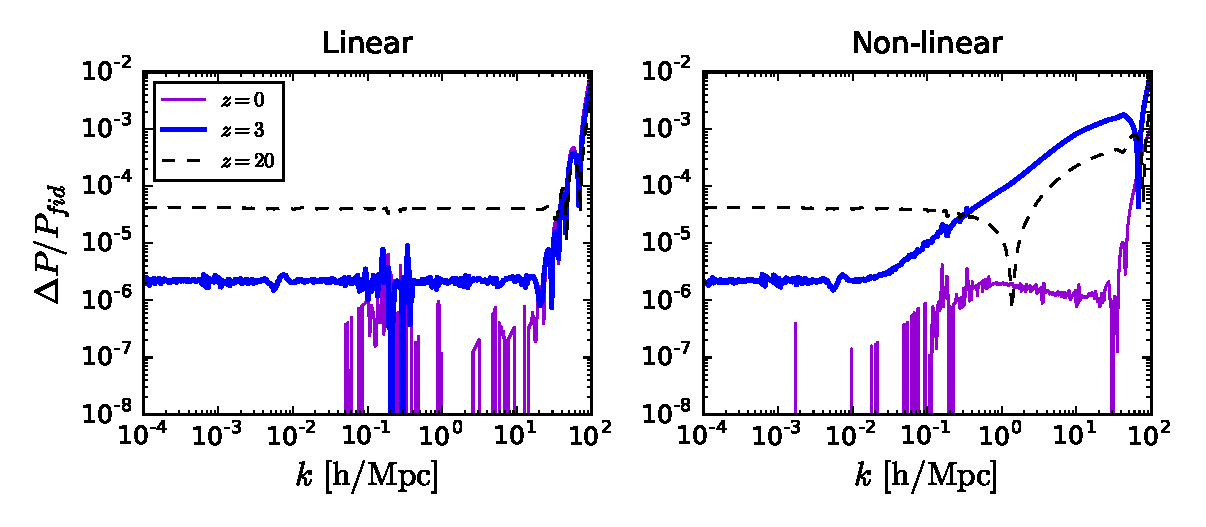
\includegraphics[width=1.0\textwidth]{plot_power.eps}
\caption{The relative error compared to power spectra produced with high values of the power spectrum splines, $P_{fid}$, produced by splining the matter power spectrum up to {\tt K$\_$MAX$\_$SPLINE} and extrapolating beyond this value with a second order Taylor expansion the natural logarithm of the matter power spectrum. The left panel shows the relative errors for the linear matter power spectrum at $z=0$, $z=3$ and $z=20$. The right panel shows the results for the non-linear matter power spectrum at the same redshifts. The standard \ccl parameters adopted are those corresponding to the black dashed curve. For comparison, the impact of baryonic physics on the matter power spectrum is $\sim 10\%$ at $k=1$/Mpc \citep{Schneider15}.}
\label{fig:NLextrapol}
\end{figure*}
%------------------------

\subsubsection{Extrapolation for the linear power spectrum}
\label{sec:Lextrapol}

With the implementation described in the previous section, the power spectrum splines are initialized up to {\tt K$\_$MAX$\_$SPLINE}. This is also true for the linear matter power spectrum, which is used within \ccl in particular to obtain $\sigma_8$ (see Eq. \ref{eq:sigR}). We have tested here how the procedure described in the previous section affects the convergence of the linear matter power spectrum. The result is shown in Figure \ref{fig:NLextrapol}. For some applications that use the linear power spectrum, the user might need to increase the value of {\tt K$\_$MAX$\_$SPLINE}.

As in the previous section, the power spectrum at small wavenumber is extrapolated using a power-law. This extrapolation is performed below a fiducial value of {\tt K\_MIN\_SPLINE} that coincides with the smallest wavenumber output by {\tt CLASS}, as in the case of the nonlinear power spectrum described above.

We have found that changing {\tt N$\_$A} to $200$, or changing the sampling of the wavenumber to $5000$ points, does not change the results presented in Figures \ref{fig:NLextrapol} in this section.

\subsubsection{Wishlist for the future}
\label{Pk_wishlist}
We plan to implement the following power spectrum methods in the future:
\begin{itemize}
 \item CAMB,
 \item other emulators,
 \item HOD.
\end{itemize}


\subsubsection{Normalization of the power spectrum}
\label{sec:PSnorm}

There are two alternative schemes for normalization of the matter power spectrum. The first one is to specify the value of $A_s$, the amplitude of the primordial power spectrum, which is passed directly to {\tt CLASS}. This option is available in the case of the linear/nonlinear matter power spectrum implementation. For these, as well as for BBKS and E\&H transfer functions, there is the additional option to set the normalization of the matter power spectrum by specifying $\sigma_8$, the RMS density contrast averaged over spheres of radius $8h^{-1}$Mpc. The computation of $\sigma_8$ is described in Section \ref{sec:hmf}.

In practice, there is only one argument that encodes the normalization. This is the argument ${\tt norm\_pk}$, which can be passed the power spectrum normalization parameterized by $\sigma_8$ or $A_\mathrm{s}$. As noted above, {\tt ccl$\_$parameters$\_$create} switches to $\sigma_8$ normalization if ${\tt norm\_pk} > 10^{-5}$, and to $A_{\mathrm s}$ normalization otherwise.

In the {\tt python} implementation, {\tt CCL} allows for either $\sigma_8$ or {\tt A\_s} to be passed as parameters.

\subsection{Angular power spectra}
\label{sec:cl}

In this section we will distinguish between {\sl observables} (quantities observed on the sky, such as number counts in a redshift bin, shear or CMB temperature fluctuations) and {\sl contributions} to the total observed fluctuations of these observables (such as the biased matter density term in number counts, redshift-space distortions, magnification, ISW, etc.).
The routines described in this subsection are implemented in {\tt ccl$\_$cls.cc}.

\subsubsection{Exact expressions}
The angular power spectrum between two observables $a$ and $b$ can be written as:
\begin{equation}
 C^{ab}_\ell=4\pi\int_0^\infty \frac{dk}{k}\,\mathcal{P}_\Phi(k)\Delta^a_\ell(k)\Delta^b_\ell(k),
\end{equation}
where $\mathcal{P}_\Phi(k)$ is the dimensionless power spectrum of the primordial curvature perturbations, and $\Delta^a$ and $\Delta^b$ are, using the terminology of CLASS, the transfer functions corresponding to these observables. Each transfer function will receive contributions from different terms. Currently \ccl supports two observables (also labelled ``tracers''), number counts and galaxy shape distortions, with the following contributions:
\paragraph{\bf Number counts.} The transfer function for number counts can be decomposed into three terms: $\Delta^{\rm NC}=\Delta^{\rm D}+\Delta^{\rm RSD}+\Delta^{\rm M}$, where
\begin{itemize}
  \item $\Delta^{\rm D}$ is the standard density term proportional to the matter density:
        \begin{equation}
          \Delta^{\rm D}_\ell(k)=\int dz\,p_z(z)\,b(z)\,T_\delta(k,z)\,j_\ell(k\chi(z)),
        \end{equation}
        where $T_\delta$ is the matter transfer function. Note that \ccl currently does not support non-linear or scale-dependent bias. Here, $p_z(z)$ is the normalized distribution of sources in redshift (selection function). Thus \ccl understands each individual redshift bin as a separate ``observable''. Note also that if ${\tt mu\_0 \ne 0}$, the matter transfer function is altered accordingly.
  \item $\Delta^{\rm RSD}$ is the linear contribution from redshift-space distortions:
        \begin{equation}
          \Delta^{\rm RSD}_\ell(k)=\int dz\,p_z(z)\frac{(1+z) p_z(z)}{H(z)}T_\theta(k,z) j_\ell''(k\chi(z)),
        \end{equation}
        where $T_\theta(k,z)$ is the transfer function of $\theta$, the divergence of the comoving velocity field. $T_\theta(k,z)$ depends on the growth, which \ccl does not compute for massive neutrino cosmologies; therefore at this time an attempt to create a number count tracer in a cosmology with massive neutrinos will cause \ccl to raise an error. $C_\ell$ is instead computed assuming a linear-theory relation between the matter overdensity and peculiar velocity fields. While this should not be problematic for wide photometric redshift bins, users should exercise care when interpreting results for narrow window functions. Note also that if the growth is affected by modifications to gravity, this is reflected here.
  \item $\Delta^{\rm M}$ is the contribution from magnification lensing:
        \begin{equation}
          \Delta_\ell^{\rm M}(k)=-\ell(\ell+1)\int \frac{dz}{H(z)} W^{\rm M}(z) T_{\phi+\psi}(k,z) j_\ell(k\chi(z)),
          \label{eq:deltaM}
        \end{equation}
        where $T_{\phi+\psi}$ is the transfer function for the Newtonian-gauge scalar metric perturbations, and $W^{\rm M}$ is the magnification window function:
        \begin{equation}
           W^{\rm M}(z)\equiv\int_z^\infty dz' p_z(z')\frac{2-5s(z')}{2}\frac{r(\chi(z')-\chi(z))}{r(\chi(z'))}.
        \end{equation}
        Here $s(z)$ is the magnification bias, given as the logarithmic derivative of the number of sources with magnitude limit, and $r(\chi)$ is the angular comoving distance (see Eq. \ref{eq:angdist}).
        
        In the case where the quasistatic parameterization of modified gravity is in use and ${\tt sigma\_0} \ne 0$, equation \ref{eq:deltaM} becomes
        \begin{equation}
          \Delta_\ell^{\rm M}(k)=-\ell(\ell+1)\int \frac{dz}{H(z)} W^{\rm M}(z) (1 + \Sigma(z)) T_{\phi+\psi}(k,z) j_\ell(k\chi(z)),
          \label{eq:deltaM}
        \end{equation}
and there is dependence on $\mu(z)$ via modifications to $T_{\phi+\psi}(k,z)$.

        Note that \ccl currently does not compute relativistic corrections to number counts \cite{2011PhRvD..84d3516C,2011PhRvD..84f3505B}. Although these should be included in the future, their contribution to the total fluctuation is largely subdominant (see \cite{GReffects} and the two references above), and therefore it is safe to work without them in most cases.
\end{itemize}

\paragraph{\bf Galaxy shape distortions.} The transfer function for shape distortions is currently decomposed into two terms: $\Delta^{\rm SH}=\Delta^{\rm WL}+\Delta^{\rm IA}$, where
\begin{itemize}
  \item $\Delta^{\rm L}$ is the standard lensing contribution:
        \begin{equation} \label{eq:transfer_lensing}
          \Delta_\ell^{\rm L}(k)=-\frac{1}{2}\sqrt{\frac{(\ell+2)!}{(\ell-2)!}}\int \frac{dz}{H(z)} W^{\rm L}(z) T_{\phi+\psi}(k,z) j_\ell(k\chi(z)),
        \end{equation}
        where $W^{\rm L}$ is the lensing kernel, given by
        \begin{equation}
          W^L(z)\equiv\int_z^\infty dz' p_z(z')\frac{r(\chi(z')-\chi(z))}{r(\chi(z'))}.
        \end{equation}
        
  When the quasistatic parameterization of modified gravity is in use, we have instead         
       \begin{equation} \label{eq:transfer_lensing}
          \Delta_\ell^{\rm L}(k)=-\frac{1}{2}\sqrt{\frac{(\ell+2)!}{(\ell-2)!}}\int \frac{dz}{H(z)} W^{\rm L}(z) (1 + \Sigma(z))T_{\phi+\psi}(k,z) j_\ell(k\chi(z)),
        \end{equation} 
        with dependence on $\mu(z)$ via $T_{\phi+\psi}(k,z)$.
  \item $\Delta^{\rm IA}$ is the transfer function for intrinsic galaxy alignments. \ccl currently supports the so-called ``non-linear alignment model'', according to which the galaxy inertia tensor is proportional the local tidal tensor \cite{2004PhRvD..70f3526H,2007MNRAS.381.1197H}.
        \begin{equation}
          \Delta_\ell^{\rm IA}(k)=\sqrt{\frac{(\ell+2)!}{(\ell-2)!}}\int dz\,p_z(z)\,b_{\rm IA}(z)\,f_{\rm red}(z)\,T_\delta(k,z)\,\frac{j_\ell(k\chi(z))}{(k\chi(z))^2}.
        \end{equation}
        Note that $\Delta_\ell^{\rm IA}(k)$ is unchanged under modified gravity other than via the matter transfer function.
\end{itemize}

It is worth noting that the equations above should be modified for non-flat cosmologies by replacing the spherical Bessel functions $j_\ell$ with their hyperspherical counterparts \cite{1994ApJ...432....7K}. Since the library currently only uses the Limber approximation (documented below), this is not currently an issue. It will be revisited in future versions of \ccl.

\paragraph{\bf CMB lensing.} The transfer function lensing convergence from a source at redshift $z_{\rm S}$ is given by:
\begin{equation} \label{eq:transfer_cmb_lensing}
  \Delta_\ell^{\rm C}(k)=-\frac{\ell(\ell+1)}{2}\int_0^{\chi_{\rm S}} d\chi\,\frac{r(\chi_{\rm S})-r(\chi)}{r(\chi)r(\chi_{\rm S})}T_{\phi+\psi}(k,\chi) j_\ell(k\chi),
\end{equation}
where $\chi_{\rm S}\equiv\chi(z_{\rm S})$. Once again under the quasistatic parameterization of modified gravity we have
\begin{equation} \label{eq:transfer_cmb_lensing}
  \Delta_\ell^{\rm C}(k)=-\frac{\ell(\ell+1)}{2}\int_0^{\chi_{\rm S}} d\chi\,\frac{r(\chi_{\rm S})-r(\chi)}{r(\chi)r(\chi_{\rm S})}(1+\Sigma(z))T_{\phi+\psi}(k,\chi) j_\ell(k\chi),
\end{equation}
with dependence on $\mu(z)$ via modifications to $T_{\phi+\psi}(k,\chi)$.

\subsubsection{The Limber approximation}
As shown above, computing each transfer function involves a radial projection (i.e. an integral over redshift or $\chi$), and thus computing full power spectrum consists of a triple integral for each $\ell$. This can be computationally intensive, but can be significantly simplified in certain regimes by using the Limber approximation, given by:
\begin{equation}
 j_\ell(x)\simeq\sqrt{\frac{\pi}{2\ell+1}}\,\delta\left(\ell+\frac{1}{2}-x\right).
\end{equation}
Thus for each $k$ and $\ell$ we can define a radial distance $\chi_\ell\equiv(\ell+1/2)/k$, with corresponding redshift $z_\ell$. This approximation works best for wide radial kernels and high multipoles.

Substituting this in the expressions above, the simplified versions become:
\begin{equation}\label{eq:limber}
 C^{ab}_\ell=\frac{2}{2\ell+1}\int_0^\infty dk\,P_\delta\left(k,z_\ell\right)
 \tilde{\Delta}^a_\ell(k)\tilde{\Delta}^b_\ell(k).
\end{equation}
where
\begin{align}
 &\tilde{\Delta}_\ell^{\rm D}(k)=p_z(z_\ell)\,b(z_\ell)\,H(z_\ell)\\
 &\tilde{\Delta}_\ell^{\rm RSD}(k)=
 \frac{1+8\ell}{(2\ell+1)^2}\,p_z(z_\ell)\,f(z_\ell)\,H(z_\ell)-\\
 &\hspace{48pt}\frac{4}{2\ell+3}\sqrt{\frac{2\ell+1}{2\ell+3}}p_z(z_{\ell+1})\,f(z_{\ell+1})\,H(z_{\ell+1})\\
 &\tilde{\Delta}_\ell^{\rm M}(k)=3\Omega_{M,0}H_0^2\frac{\ell(\ell+1)}{k^2}\,
 \frac{(1+z_\ell)}{r(\chi_\ell)}W^{\rm M}(z_\ell)\\
 &\tilde{\Delta}_\ell^{\rm L}(k)=\frac{3}{2}\Omega_{M,0}H_0^2\sqrt{\frac{(\ell+2)!}{(\ell-2)}}\frac{1}{k^2}\,
 \frac{1+z_\ell}{r(\chi_\ell)}W^{\rm L}(z_\ell)\\
 &\tilde{\Delta}_\ell^{\rm IA}(k)=\sqrt{\frac{(\ell+2)!}{(\ell-2)!}}\frac{p_z(z_\ell)\,b_{\rm IA}(z_\ell)f_{\rm red}(z_\ell)H(z_\ell)}{(\ell+1/2)^2}\\
 &\tilde{\Delta}_\ell^{\rm C}(k)=\frac{3}{2}\Omega_{M,0}H_0^2\,\ell(\ell+1)\frac{1+z_\ell}{k^2}\,\frac{r(\chi_{\rm S})-r(\chi_\ell)}{r(\chi_\ell)r(\chi_{\rm S})}\,\Theta(\chi_\ell;0,\chi_{\rm S}).
\end{align}
Here ($\Theta(x;x_i,x_f)$) is a top-hat function (1 for $x\in[x_i,x_f]$ and 0 otherwise).

%----------------------------------------------------------------
%
%      Begin of the Angpow section currently under development
%
%----------------------------------------------------------------

\subsubsection{Beyond limber}

{\bf Native CCL computation.}

\ccl incorporates routines to compute the $C^{ab}_\ell$ angular power spectra as described above but without the Limber approximation. The algorithm performs first the integrals over $z$ for both tracers, and ends with the $k$ integral. This computation is much slower than using the Limber approximation, but it ends up with precise angular power spectra at low $\ell$, and correct cross-correlations between tracers (the Limber approximation fails at reproducing the interference terms $j_\ell(x)\times j_\ell(x')$).

Some parameters are needed to define this integral. First, to fasten the computation the $C^{ab}_\ell$ function is computed for a selection of $\ell$ values (linearly spaced at low-$\ell$ and logarithmicly spaced at high-$\ell$) and then the function is splined. Then the integration step of the redshift integrals must be specified in terms of a comoving distance. It is recommanded to start with a low value ($<3$\,Mpc) for a high precision integration, and then to release this parameter to achieve the user needs in terms of precision and rapidity. A logarithmic step in $k$ must also be provided: it does not correspond to the integration step but to a computation step before splining the transfer functions $\Delta^a_\ell(k)$. Last parameter, a minimum redshift can be given for the redshift integral bound so that the transfer functions are not computed near $z\approx 0$ where they can be numerically undefined.

The integration bounds in redshift are estimated automatically given the a redshift window so that the integration is preformed where the redshift window is relevant within a given precision (set by the \texttt{CCL\_FRAC\_RELEVANT} parameter). The integration bounds for the $k$ integrals are defined automatically given the $\ell$ multipole and the comoving distances at play.

It is worth noting that the user can define a threshold multipole $\ell$ from which the $C^{ab}_\ell$ computation switches to the Limber approximation which is faster and generally relevant at high $\ell$ values. 

{\texttt{\bf Angpow}.}

The aim of the \texttt{Angpow} software \citep{2017arXiv170103592C} is to compute the angular power spectra  $C_{\ell}^{ab}$  without any Limber numerical approximation. \ccl has been linked to the \texttt{Angpow} code,  which is briefly described here.

The angular power spectrum for two shells $C_{\ell}^{ab}$ is computed in \texttt{Angpow} according to the following expression
\begin{equation}
  C_{\ell}^{ab} = \iint_0^\infty \mathrm{d} z \mathrm{d} z^\prime  p_{z_1}(z_1) p_{z_2}(z^\prime) \times \int_0^\infty \mathrm{d} k\ f_{\ell}(z, k) f_{\ell}(z^\prime, k).
  \label{eq-clz1z2-obs}
\end{equation}
The auxiliary function $f_\ell(z,k)$ can be defined without loss of generality as
\begin{equation}
f_\ell(z,k) \equiv  \sqrt{\frac{2}{\pi}}\  k \sqrt{P(k,z)}\ \widetilde{\Delta}_\ell(z,k)\label{eq-fell-func}
\end{equation}
with
\begin{itemize}
\item  $P(k,z)$ : the matter power spectrum at redshift $z$ 
\item $\widetilde{\Delta}_\ell(z,k)$: a function describing the physical processes such as matter density fluctuations, redshift-space distortions as described for instance in references \citet{2008cmb..book.....D,2009PhRvD..80h3514Y,2010PhRvD..82h3508Y, 2011PhRvD..84d3516C,2011PhRvD..84f3505B}. Currently, the \texttt{Angpow} version delivered with \ccl only can deal with galaxy clustering tracers (no lensing) and this without the magnification lensing term (equation \ref{eq:deltaM}). The incorporation of those transfer functions is left for future work, but in principle \texttt{Angpow} has already the capability to treat them. For now, for galaxy clustering tracers we defined $\widetilde{\Delta}_\ell(z,k)$ as 
\begin{equation}
 \widetilde{\Delta}_\ell(z,k) \approx b j_\ell(k \chi(z)) - f(z) j_\ell^{\prime\prime}(k \chi(z)) 
\end{equation}
with $j_\ell(x)$ and $j_\ell^{\prime\prime}(x)$ the spherical Bessel function of order $\ell$ and its second derivative, and $f(a)$ the growth rate as defined subsection~\ref{sec:growth} (derivative of the growth function with respect to the scale factor $a$).
\end{itemize}

To proceed to a numerical evaluation of equation \ref{eq-clz1z2-obs}, \texttt{Angpow} first conducts  inside the rectangle $ [z_{1\mrm{min}},z_{1\mrm{max}}] \times [z_{2\mrm{min}},z_{2\mrm{max}}]$ given by the $p_z(z)$ selection functions a Cartesian product of one-dimensional (1D) quadrature
 defined by the set of sample nodes $z_i$ and weights $w_i$. In practice, the Clenshaw-Curtis quadrature is used.   The corresponding sampling points $(z_{1i},z_{2j})$ are weighted by the product  $w_i w_j$ using the 1D quadrature sample points and weights on both redshift regions with $i=0,\dots, N_{\mrm{z}_1}-1$ and $j=0,\dots,N_{\mrm{z}_2}-1$. Then, one gets the following approximation:
\begin{equation}
C_{\ell}^{ab} \approx  \sum_{i=0}^{N_{\mrm{z}_1}-1}\sum_{j=0}^{N_{\mrm{z}_2}-1} w_i w_j p_{z_1}(z_i)p_{z_2}(z_j) \widehat{P}_\ell(\chi_i,\chi_j)
\label{eq-cross-zquadra}
\end{equation}
with the notations $z_i = z_{1i}$, $z_j = z_{2j}$ and  $\chi_i = \chi(z_{1i})$, $\chi_j = \chi(z_{2j})$ and
\begin{equation}
\widehat{P}_\ell(z_i,z_j) =   \int_0^\infty dk\ f_\ell(z_i,k) f_\ell(z_j,k)
\label{eq-Pellzizj}
,\end{equation}
To conduct the computation of such integral of highly oscillating functions we use the 3C-algorithm described in details in reference \citep{2017arXiv170103592C}. In brief this algorithm proceeds the following way:
\begin{enumerate}
\item the total integration $k$ interval (eg. $[k_\mathrm{min}, k_\mathrm{max}]$) in equation (\ref{eq-Pellzizj}) is cut on several $k$-sub-intervals;
\item  on each sub-interval the functions $f_{i\, \ell}(k) = f_\ell(z_i,k) $ and $f_{j\, \ell}(k) = f_\ell(z_j,k)$ are projected onto Chebyshev series of order $2^N$;
\item the product of the two Chebyshev series is performed with a $2^{2N}$ Chebyshev series;
\item then, the integral on the sub-interval is computed thanks to the Clenshaw-Curtis quadrature.
\end{enumerate}
All the Chebyshev expansions and the Clenshaw-Curtis quadrature are performed via the DCT-I fast transform of FFTW.

Thanks to the 3C-algorithm, the \texttt{Angpow} is able to compute the $C_{\ell}^{ab}$ in a fast and accurate way. It was tested against \texttt{CLASS} and the native \ccl computation and can performed the computation an order of magnitude faster, which is more suitable for an extensive exploration of the cosmological parameter space ($\mathcal{O}(1s)$). Note that \texttt{Angpow} is written in C++ with OpenMP, to distribute the computation of a single $C_\ell$ on a single thread. The computation can also be switch by the user to the faster Limber approximation setting a threshold multipole $\ell$.
 

{\bf Precision tests.}

The code has been compared with \texttt{CLASS} and the native \ccl computation and all three softwares agrees perfectly if precision parameters are pushed to high levels.

A few parameters must be provided to set the precision of this computation. First the order of the Chebyshev polynomials is set to $2^{10}$ by default, and the number of $k$ sub-intervals to 200, and we checked this is enough for the current uses. Then the redshift quadrature stepping is set automatically given the redshift windows to recover the native \ccl computation boosted with high precision parameters: its precision is optimised so that the relative numerical error compared with the native method is two orders of magnitude below the relative cosmic variance $\sqrt{2/(2\ell+1)}$, from $\ell=2$ to $\ell=1000$. The $k_{\rm min}$ and $k_{\rm max}$ bounds are also automatically set given the current multipole $\ell$ and the comoving distance $\chi$ involved in the inner integral.




%----------------------------------------------------------------
%
%      End of the Angpow section currently under development
%
%----------------------------------------------------------------

\subsection{Correlation functions}
\label{sec:corr}


The following expressions relating the angular power spectra and correlation functions are valid in the flat-sky approximation\footnote{See the weak lensing review by \citet{Bartelmann01}, page 44 and \citet{Joachimi10}.}. In all cases, $f_K(\chi)$ is comoving angular diameter distance, which differs from the radial comoving distance $\chi$ only in the case of cosmologies with non-zero curvature. The routines described in this subsection are implemented in {\tt ccl$\_$correlation.c}.

{\bf Galaxy-galaxy.} The angular correlation function between two number-count tracers (labeled $a$ and $b$ here) is given by
\begin{equation}
  \xi^{ab}(\theta) = \int d\ell \frac{\ell}{2\pi} C^{ab}_\ell\, J_0(\ell\theta),
\label{eq:xiclu}
\end{equation}
where $C_{ab}$ is the angular power spectrum between both tracers.

{\bf Lensing-lensing.} The lensing correlation functions are \footnote{from Schneider 2002 and Bartelmann \& Schneider section 6.4.1}
\begin{eqnarray}
  \xi^{ab}_{+}(\theta)&=&\int_0^{\infty}d\ell\frac{\ell}{2\pi}J_0(\ell\theta)C^{ab}_\ell,\\
  \xi^{ab}_{-}(\theta)&=&\int_0^{\infty}d\ell\frac{\ell}{2\pi}J_4(\ell\theta)C^{ab}_\ell,
\label{eq:xipxim}
\end{eqnarray}
where the angular lensing convergence power spectrum $C^{ab}_\ell$ is given above (see Equations \ref{eq:transfer_lensing} and \ref{eq:limber}).

{\bf Galaxy-lensing.} The correlation between a number count tracer $a$ and a shear tracer $b$ is given by
\begin{equation}
  \xi^{ab}(\theta) = \int d\ell \frac{\ell}{2\pi} C^{ab}_\ell\, J_2(\ell\theta),
\end{equation}

Note that, in the above, ``Galaxy'' and ``Lensing'' can be replaced by any spin-0 and spin-2 fields on the sphere respectively (e.g. the CMB lensing convergence would play the same role as the galaxy overdensity field in all the formulas above).

{\bf 3d spatial correlation function.} In addition to the angular correlation functions, the 3-dimensional spatial correlation function $\xi(r)$ is also 
calculated from the power spectrum $P(k)$ using
\begin{equation}
\xi(r) = \frac{1}{2 \pi^2} \int dk \; k^2 P(k) \frac{\sin(kr)}{kr}
\end{equation}


To evaluate the numerical integral in the correlation functions, we make use of the public code {\tt FFTlog}\footnote{\url{http://casa.colorado.edu/~ajsh/FFTLog/}}\citep{Hamilton2000,Talman2009}. In brief, {\tt FFTlog} works on functions periodic in log space, by writing the Hankel Transform as a convolution between Bessel functions and the function of interest (in this case either $C_\ell$ or $P(k)$). A version of this code is included in \ccl with minor modifications.

%-----------------------------------------------------------
%
%   Correlation: beyond flat-sky (under development)
%
%-----------------------------------------------------------

\begin{comment}
\subsubsection{Beyond flat-sky}

We begin by writing the angular space observable, $X$, in terms of a decomposition in spherical harmonics,
\begin{align}\label{eq:X_harmonic}
  X(\Omega)=&\sum_{\ell m}\tilde X_{\ell m}Y_{\ell m}(\Omega)
\end{align}
where $\Omega$ refers to the angular coordinates on the sky.
The angular cross correlation function of two (scalar) tracers, $X$ and $Z$ of the large scale structure can be written in terms of their harmonic components, $\tilde X_{\ell m}$ and $\tilde Z_{\ell' m'}$ as
\begin{align}
  \langle XZ \rangle(\theta)=&\left\langle\sum_{\ell,m}\sum_{\ell', m'}\tilde X_{\ell m}\tilde Z_{\ell' m'}
  Y_{\ell m}(\Omega)
  Y_{\ell'm'}(\Omega+\theta)\right\rangle\\
  =&\sum_{\ell,m}C_{\ell}Y_{\ell m}(\Omega)
  Y_{\ell m}(\Omega+\theta)\\
  \langle XZ \rangle(\theta)=&\frac{1}{4\pi}\sum_{\ell}(2\ell+1)C_{\ell}P_{\ell}(\cos\theta)\label{eq:xi_pl0}
\end{align}
where we have used the identities
\begin{align}
  \langle\tilde X_{\ell m}\tilde Z_{\ell' m'}\rangle=&C_{\ell}\delta_D(m,m')\delta_D(\ell,\ell'),\\
  \sum_{m=-\ell}^{m=\ell}Y_{\ell m}(\Omega)Y_{\ell m}(\Omega+\theta)=&\frac{2\ell+1}{4\pi}\label{eq:Ylm_Pl}.
\end{align}

For the case of shear, since it is a spin-2 object, eq.\ref{eq:X_harmonic} is written in terms of spin harmonics
\citep[see for ex.][]{Castro2005,Kilbinger2017}. The rest of the analysis proceeds similarly, using the relation for spin
harmonics, analogous to eq.~\ref{eq:Ylm_Pl} \citep[see for ex. ][]{Hu1997}.

The expressions for $\xi_+$ (which is the same as in Eq.~\ref{eq:xi_pl0}) and for $\xi_-$ are given by
\begin{align}
  %\langle g\gamma_T\rangle(\theta)&=\frac{1}{4\pi}\sum_{\ell}\frac{(2\ell+1)}{\ell(\ell+1)}C_{\ell}^{g\kappa}
  %P_{\ell}^2(\cos\theta)\label{eq:xi_g_gamma}\\
  \xi_+(\theta)&=\frac{1}{4\pi}\sum_{\ell}{(2\ell+1)}C_{\ell}^{\kappa\kappa}
  P_{\ell}(\cos\theta)\label{eq:xi_p}\\
  \xi_-(\theta)&=\frac{1}{4\pi}\sum_{\ell}\frac{(\ell-4)!}{(\ell+4)!}\ell^4{(2\ell+1)}C_{\ell}^{\kappa\kappa}
  P_{\ell}^4(\cos\theta)\label{eq:xi_m}
\end{align}
\todo{Simply took the relation between $P_\ell^m$ and $J_m(\ell \theta)$ to get this expression from the Hankel transform for $\xi_-$. It may not be very accurate at large scale (low $\ell$) as is evident from $g\gamma_T$ expression. To be revisited.}

The {\tt ccl\_tracer\_corr\_legendre} routine computes these transform to convert angular power spectra, $C_\ell$, into correlation functions. We use the associated Legendre function implementation from the {\tt GSL} library. {\tt ccl\_tracer\_corr\_legendre} routine evaluations can be very slow, especially for polynomials $P_\ell^m$ with $m>0$. Note that $P_\ell^m$ evaluations need to be done only once and can then be saved as long as $\ell$ and $\theta$ values do not change. However, \ccl has not yet implemented this feature.

\paragraph{Hankel Transform}
Notice that in the flat-sky limit, the expressions in Eqs.~\ref{eq:xi_p}--\ref{eq:xi_m} can be written as Hankel transforms using the relation between $P_{\ell}^m$ and bessel functions $J_m$
\begin{align}
  P_{\ell}^m(\cos\theta)=(-1)^m\frac{(\ell+m)!}{(\ell-m)!}\ell^{-m}J_m(\ell\theta)
\end{align}
which yields final expressions that coincide with Eq. \ref{eq:xipxim}.

\end{comment}


%-----------------------------------------------------------
%
%   End of Correlation: beyond flat-sky (under development)
%
%-----------------------------------------------------------


\subsection{Halo mass \& halo bias functions}
\label{sec:hmf}

The routines described in this subsection are implemented in {\tt ccl$\_$massfunc.c}.

The halo mass function is implemented using several different definitions from the literature: \citet{Tinker2008}, \citet{Tinker2010}, \citet{Angulo2012}, and \citet{Watson2013}. All four models are tuned to simulation data and tested against observational results. In addition, each of these fits has been implemented using the common halo definition of $\Delta = 200$, where a halo is defined with:
\begin{equation}
\bar{\rho}(r_{\Delta}) = \Delta \times \rho_{\mathrm{m}},
\end{equation}
where a halo with size $r_{\Delta}$ has an average density $\bar{\rho}$ equal to the overdensity parameter $\Delta$ times the mean background density of the universe, $\rho_{\mathrm{m}}$. Note that another common definition utilizes the critical density of the universe, $\rho_{\mathrm{c}}$; currently \ccl requires that an external conversion by the end user between values of $\Delta$ with respect to the critical density to values of $\Delta$ as defined with respect to the mean density. In the future we plan to allow for self-consistent handling of critical density based definitions, though it is not implemented as of this build.

In addition to the usage of the most common definition, we have implemented an extension for two of the models. The Tinker 2010 model allows for a value of $\Delta$ to be given between the values of 200 and 3200 and interpolates the fitting parameters within this range in a space of $\log \Delta$ using splines. We also have implemented interpolation in the same range of Tinker 2008 $\Delta$ values. For both Tinker 2008 and Tinker 2010 models we have utilized spline interpolation through {\tt GSL} routines in order to guarantee a match to specified fitting parameters at exact values of $\Delta$. This fitting has slight deviation from the fit as expressed in Tinker 2010.

The halo mass function models implemented in CCL are tuned to simulations without massive neutrinos, therefore are not valid in cosmologies with massive neutrinos. Attempts to calculate the halo mass function, halo bias, or other related quantities within cosmologies with massive neutrinos will cause \ccl to raise an error and quit.


With the exception of the Tinker 2010 model, we attempt to keep a common form to the multiplicity function whenever possible for ease of extension:
\begin{equation}
f(\sigma)=A\Big[\Big(\frac{\sigma}{b}\Big)^{-a}+1\Big]e^{-c/{\sigma}^2},
\end{equation}
where $A$, $a$, $b$, and $c$ are fitting parameters that have additional redshift scaling and $\sigma$ is the RMS variance of the density field smoothed on some scale $M$ at some scale factor $a$. This basic form is modified for the \citet{Angulo2012} formulation. The resulting form is
\begin{equation}
f(\sigma)=A\Big[\Big(\frac{b}{\sigma}+1\Big)^{-a}\Big]e^{-c/{\sigma}^2},
\end{equation}
where the only change is in the formulation of the second term. Note that the fitting parameters in the \citet{Angulo2012} formulation do not contain any redshift dependence and the use of it is primarily for testing and benchmark purposes.

Each call to the halo mass function requires an assumed model (defined within the {\tt ccl$\_$configuration} structure contained in {\tt ccl$\_$cosmology}), in addition to a value of the halo mass and scale factor for which to evaluate the halo mass function. The currently implemented models can be called with the tags {\tt config.mass$\_$function$\_$method = ccl$\_$tinker}, {\tt ccl$\_$tinker10}, {\tt ccl$\_$angulo}, or {\tt ccl$\_$watson}. It returns the number density of halos in logarithmic mass bins, in the form $dn/d\log_{10}{M}$, where $n$ is the number density of halos of a given mass and $M$ is the input halo mass.

The halo mass $M$ is related to $\sigma$ by first computing the radius $R$ that would enclose a mass $M$ in a homogeneous Universe at $z=0$:
\begin{equation}
  M=\frac{H_0^2}{2G}R^3\,\rightarrow \frac{M}{M_\odot}=1.162\times10^{12}\Omega_Mh^2\,\left(\frac{R}{1\,{\rm Mpc}}\right)^3.
\end{equation}
The rms density contrast in spheres of radius $R$ can then be computed as
\begin{equation}
  \sigma_R^2 = \frac{1}{2\pi^2}\int dk\,k^2\,P_k\,\tilde{W}_R^2(k)
  \label{eq:sigR}
\end{equation}
where $P_k$ is the matter power spectrum and $\tilde{W}(kR)$ is the Fourier transform of a spherical top hat window function,
\begin{equation}
\tilde{W}_R(k) = \frac{3}{(kR)^3}[\sin(kR)-kR\cos(kR)]
\end{equation}
%
This function is directly implemented in \ccl as well as a specific $\sigma_8$ function.

The \citet{Tinker2010} model parameterizes both the halo mass function and the halo bias in terms of the peak height, $\nu = \delta_c / \sigma(M)$, where $\delta_c$ is the critical density for collapse and is chosen to be $1.686$ for this particular parameterization. We can then parameterize the halo function and halo bias as
\begin{equation}
  b(\nu) = 1 - A\frac{\nu^a}{\nu^a + {\delta_c}^a} + B\nu^b+C\nu^c,
  f(\nu) = \alpha[1+(\beta\nu)^{-2\phi}]\nu^{2\eta}e(-\gamma\nu^2/2).
\end{equation}
The currently implemented model in \ccl allows for an arbitrary overdensity $\Delta$ to be chosen, using the fitting functions provided in \citet{Tinker2010}. Other halo model definitions are not included in the halo bias calculation, though this remains an area of active work to improve upon.

The halo mass function and related quantities

\subsection{Photo-$z$ implementation}
\label{sec:photoz}
The functionality described in this section is implemented in {\tt ccl\_lsst\_specs.c}.

LSST galaxy redshifts will be obtained using photometry. A model is therefore required for the probability of measuring a photometric redshift $z_{\rm ph}$ for an object with hypothetical spectroscopic redshift $z_{\rm s}$. \ccl allows the user to flexibly provide their own photometric redshift model.

To take advantage of this functionality, the user writes a function which accepts as input a photometric redshift, a spectroscopic redshift, and a void pointer to a structure containing any further parameters of the photo-z model. This function will return the probability of measuring the input photometric redshift given the input spectroscopic redshift. Explicitly, it should take the form:

{\tt user$\_$pz$\_$probability(double z$\_$ph, double z$\_$s, void * user$\_$par)\{...\}}

This function is responsible for extracting the photo-z model parameters from the void pointer {\tt user$\_$par} itself.

This model can be used when computing $\frac{dN}{dz}^i$ in photometric redshift bin $i$, as given by equation \ref{photoz} below. An example of how the user can construct the required functions and structure can be found in {\tt ccl\_sample\_run.c}. An example that uses a built-in Gaussian photo-z model is also provided.

\subsection{LSST Specifications}
\label{sec:specs}

\ccl includes LSST specifications for the expected galaxy distributions of the full galaxy clustering sample and the lensing source galaxy sample. These enable the user to easily make forecasts for LSST. The functionality described in this section is implemented in {\tt ccl\_lsst\_specs.c}.

The functional forms of the expected $\frac{dN}{dz}$ for clustering galaxies and lensing source galaxies are provided. Here, $\frac{dN}{dz}$ is the number density of galaxies as a function of true redshift.

In the case of lensing source galaxies, these forms are given in \cite{Chang2013}, wherein three different cases are considered: fiducial, optimistic, and conservative. All three are included in \ccl, and are indicated via a label of {\tt DNDZ$\_$WL$\_$OPT}, {\tt DNDZ$\_$WL$\_$FID}, and {\tt DNDZ$\_$WL$\_$CONS} as appropriate. The functional form of $\frac{dN}{dz}$ for lensing source galaxies is given as:
\begin{equation}
\frac{dN}{dz} \propto z^\alpha {\rm exp}\left(-\frac{z}{z_0}^\beta\right).
\label{dndz_src}
\end{equation}
The parameters, in the fiducial case, are given as $\alpha=1.24$, $\beta=1.01$, and $z_0=0.51$. In the optimistic case, this becomes $\alpha=1.23$, $\beta=1.05$, and $z_0=0.59$. The conservative case is given by $\alpha=1.28$, $\beta=0.97$, and $z_0=0.41$.

For the case of the clustering galaxy sample, the functional form is given by \citep{ScienceBook}:
\begin{equation}
\frac{dN}{dz} \propto \frac{1}{2z_0}\left(\frac{z}{z_0}\right)^2 {\rm exp}\left(-\frac{z}{z_0}\right)
\label{dndz_clust}
\end{equation}
with $z_0=0.3$.

In order to be incorporated into forecasts or predictions, the above expressions for $\frac{dN}{dz}$ must be normalized, and the value of $\frac{dN}{dz}$ must be provided in a given photometric redshift bin. Support is provided for the user to input a flexible photometric redshift model, as described in Section \ref{sec:photoz}. This takes the form of a function which returns the probability $p(z,z')$ of measuring a particular photometric redshift $z$, given a spectroscopic redshift $z'$ and other relevant parameters. Also provided are functions to return $\sigma_z$ at a given redshift for both lensing sources and clustering galaxies, for the case in which the user-defined function is a Gaussian photo-z model.

With this, $\frac{dN^i}{dz}$ of lensing or clustering galaxies in a particular photometric redshift bin $i$ is given by:
\begin{equation}
\frac{dN^i}{dz} = \frac{\frac{dN}{dz}\int_{z_i}^{z_{i+1}} dz' p(z,z')}{\int_{z_{\rm min}}^{z_{\rm max}}dz \frac{dN}{dz} \int_{z_i}^{z_{i+1}}dz' p(z, z')}
\label{photoz}
\end{equation}
where $z_{i}$ and $z_{i+1}$ are the photo-z edges of the bin in question.

Finally, the expected (linear, scale-independent) bias of galaxies in the clustering sample is also provided. It is given by \citep{ScienceBook}:
\begin{equation}
b(z) = \frac{0.95}{D(z)}
\label{clustbias}
\end{equation}
where $D(z)$ in the linear growth rate of structure normalized to unity at z=0. Note that this bias definition requires the calculation of the linear growth rate and therefore is not yet supported for cosmologies with massive neutrinos.

\section{Tests and validation}
\label{sec:tests}

Our goal is for outputs of \ccl to be validated against the results of a code-comparison project run within LSST-DESC down to a $10^{-4}$ or pre-established accuracy level if possible. In some cases, this level of accuracy is not necessary, as other systematics which have not been considered in this version of \ccl yet are expected to have a larger fractional impact. In the cases where this applies, we make it clear below.


A code comparison project was carried out among members of TJP where the following outputs of cosmological forecast codes were compared and validated:
\begin{enumerate}
\item growth factor at $z = 0,1,2,3,4,5$,
\item comoving radial distance $[$Mpc$/h]$ at the same redshifts, as well as the corresponding distance moduli,
\item linear matter power spectrum, $P(k)$, from BBKS \citep{BBKS} in units of $($Mpc$/h)^3$ at $z=0,2$ in the range $10^{-3} \leq k \leq 10 h/$Mpc with 10 bins per decade,
\item Eisenstein \& Hu matter power spectrum in units of $($Mpc$/h)^3$ at $z=0$ in the range $10^{-3} \leq k \leq 10 h/$Mpc with 10 bins per decade, and
\item the mass variance at $z=0$, $\sigma(M,z=0)$ for $M =\{10^6, 10^8, 10^{10}, 10^{12}, 10^{14}, 10^{16}\} $M$_\odot/h$.
\end{enumerate}
These predictions were produced and compared for different cosmologies, which are listed in the table below. The results agree to better than $0.1\%$ relative accuracy for comoving distance and growth factor among all submissions, and for $P(k)$ and $\sigma(M)$ among codes which use the same BBKS conventions.

\begin{table}
\begin{center}
  \begin{tabular}{ c | c c c c c c c c }
%    \hline
%    \multicolumn{9}{|c|}{Cosmological models for code comparison project} \\
    \hline
    \hline
    Model & $\Omega_m$ & $\Omega_b$ & $\Omega_\Lambda$ & $h_0$ & $\sigma_8$ & $n_s$ & $w_0$ & $w_a$ \\
    \hline
    flat LCDM & 0.3 & 0.05 & 0.7 & 0.7 & 0.8 & 0.96 & -1 & 0 \\
    $w_0$ LCDM & 0.3 & 0.05 & 0.7 & 0.7 & 0.8 & 0.96 & -0.9 & 0  \\
    $w_a$ LCDM & 0.3 & 0.05 & 0.7 & 0.7 & 0.8 & 0.96 & -0.9 & 0.1  \\
    open $w_a$ LCDM & 0.3 & 0.05 & 0.65 & 0.7 & 0.8 & 0.96 & -0.9 & 0.1  \\
    closed $w_a$ LCDM & 0.3 & 0.05 & 0.75 & 0.7 & 0.8 & 0.96 & -0.9 & 0.1  \\
    \hline
	\end{tabular}
	\caption{Cosmological models for the code comparison project.}
    \label{table:code_comp}
\end{center}
\end{table}
We noticed that there are 2 typos for the BBKS transfer function in ``Modern Cosmology'' \citep{DodelsonBook} compared to the original BBKS paper. The quadratic term should be $(16.1q)^2$ and the cubic term should be $(5.46q)^3$. The BBKS equation is correct in \citet{PeacockBook}. Using the wrong equation can give differences in the results above the $10^{-4}$ level.

From the comparison, we were also able to identify some typical issues which affect convergence at the desired level:
\begin{itemize}
\item For achieving $10^{-4}$ precision in $\sigma(M)$ and the normalisation of the power spectrum, one should check that the integral of $\sigma_8$ and $\sigma(M)$ has converged for the chosen values of $\{k_{\rm min},k_{\rm max}\}$. After checking convergence, we achieved the desired precision.
\item Also note that for $\sigma(M)$, it is important to set the desired precision level correctly for the numerical integrator. The integral usually yields $\sigma^2(M)$, and not $\sigma(M)$. Hence, one has to set the desired precision taking the exponent into account.
\item The value of the gravitational constant, $G$, enters into the critical density. We found that failure to define $G$ with sufficient precision would result in lack of convergence at the $10^{-4}$ level between the different submissions. Importantly, note that CAMB barely has $10^{-4}$ precision in $G$ (and similarly, there might be other constants within CAMB/CLASS for which one should check the precision level). For \ccl, we are using the value from the Particle Physics Handbook.
\item Including/excluding radiation in the computation of the comoving distances and the growth function can easily make a difference of $10^{-4}$ at the redshifts required in this comparison.
\end{itemize}

In a second stage, we used the BBKS linear matter power spectrum from the previous step to compare two-point statistics for two redshift bins, resulting in three tomography combinations, ($1-1$),($1-2$),($2-2$). We computed the following quantities:
\begin{itemize}
\item projected galaxy clustering tomography power spectra: density term only (no magnification, RSD, etc.) with non-evolving linear bias $b(z) = 1$, in the range $10 < \ell < 10000$, using $5$ bins per decade,
\item angular convergence tomography power spectra: leading order convergence term only (no magnification), in the same range and with the same resolution as the case above,
\item angular galaxy clustering tomography correlation function, in the range $0.01 \deg < \theta < 5 \deg$, using 5 bins per decade, and
\item angular shear tomography correlation functions ($\xi_+$,$\xi_-$), similarly to above.
\end{itemize}
We adopted the following analytic redshift distributions: a Gaussian with $\sigma = 0.15$, centered at $z_1 = 1$; and another Gaussian with the same dispersion but centered at $z_2 = 1.5$. We repeated the exercise for two redshift distribution histograms shown in Figure \ref{fig:zhistos}.

%------------------------
\begin{figure}
\centering
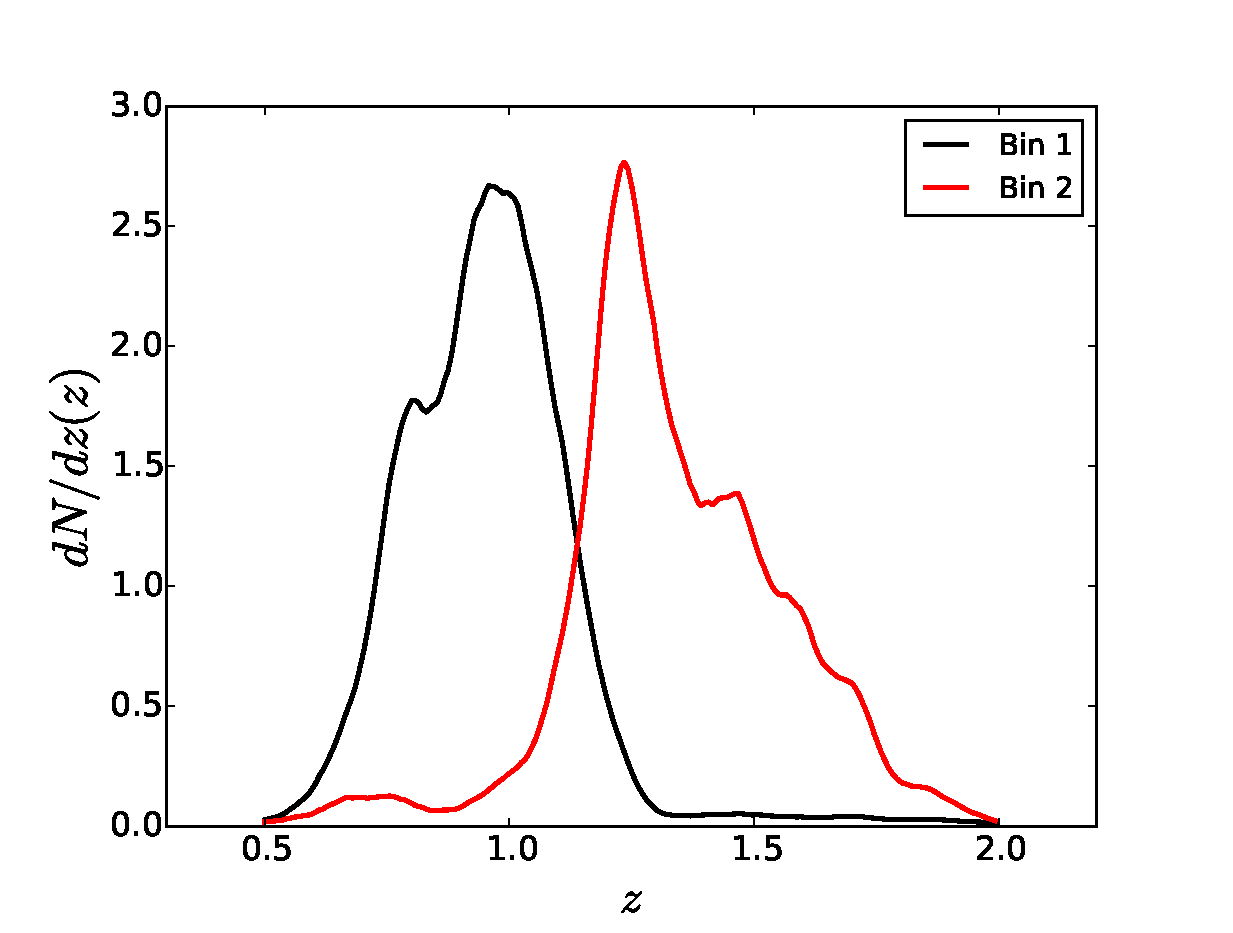
\includegraphics[width=0.6\textwidth]{zdist.eps}
\caption{Binned redshift distributions used for code comparison project.}
\label{fig:zhistos}
\end{figure}
%------------------------

In this second step, only 2 codes have been compared so far. More outputs are needed to guarantee convergence. Preliminarily, from these outputs, we have concluded that:
\begin{itemize}
\item The cross-correlation between bins is particularly sensitive to the number of points where the kernels have been sampled.
\item The accuracy of the correlation function is sensitive to $\ell_{\rm max}$. We had to use up to $\ell_{\rm max}=3\times10^4$ for convergence (and we could not achieve $0.01\%$ convergence).
\item The large scales of the correlation function are sensitive to $\ell_{\rm min}$. The use of the flat-sky approximation is also relevant on these scales.
\item For sufficiently high precision, the correlation functions are sensitive to how the power spectrum is sampled and interpolated.
\end{itemize}

For $C_\ell$ computations, we required the relative difference between \ccl and the benchmarks to be $<10^{-3}$. We performed the test both for analytic redshift distributions and histograms.

To obtain realistic targets for the convergence of correlation function computations for LSST analyses, we calculate the expected statistical uncertainty of the clustering and lensing correlation functions of the LSST gold sample (c.f. Sect.~\ref{sec:specs}), assuming an effective source galaxy density of $n_\mathrm{eff} = 26\mathrm{gal/sq\,arcmin}$ for galaxy shape distortions, and galaxy density of $n_\mathrm{gold} = 45\mathrm{gal/sq\,arcmin}$ for number counts. Specifically, we calculate the Gaussian covariance of angular correlation functions following the formalism of \citet{2008A&A...477...43J}, and note that leaving out the non-Gaussian covariance terms makes this convergence criterion more conservative. We split the galaxy samples into 10 tomography bins, defined to contain equal numbers of galaxies. The accuracy test then proceeds as follows. We compared the difference between \ccl calculated lensing and clustering correlations and the benchmarks for the analytic redshift distributions and for auto-correlations of redshift bins only. To pass the benchmark test, we required that this difference be smaller than half of the value of the errorbar derived from the covariance for each correlation function computed. Specifically, we take the value of the covariance in the bins centered at $z=1$ and $z=1.5$ to compare to the benchmarks.

The 3-dimensional correlation function $\xi(r)$ was validated by comparing with an independent, precise numerical transform. We calculated $\xi(r)$ 
by transforming the CCL non-linear Halofit power spectrum using this independent code for the five cosmologies listed in Table~\ref{table:code_comp} at 
redshifts $z = 0,1,2,3,4,5$.  We then compared with the $\xi(r)$ from CCL with a sampling of $P(k)$ 
equal to {\tt N$\_$K$\_$3DCOR} bins per decade. The default value of {\tt N$\_$K$\_$3DCOR}~=~100,000 results in a relative agreement 
at the level of $\Delta \xi(r) / \xi(r) < 2.5 \times 10^{-3}$ for $0.1 < r < 250$~Mpc and redshift zero. The agreement is better for higher redshifts.
We also compared the absolute value of $r^2 \xi(r)$ and find a maximum difference of $\Delta (r^2 \xi(r)) < 3.0 \times 10^{-2}$ for the range 
$r = 0.1 - 250$~Mpc. This corresponds to approximately 0.08\% of the BAO peak value of $r^2 \xi(r)$. At the BAO peak, the difference is 
only $9.0 \times 10^{-3}$, or 0.024\% of the peak height. The results are shown in Fig.~\ref{fig:benchmark_xi}
%
\begin{figure*}
\centering
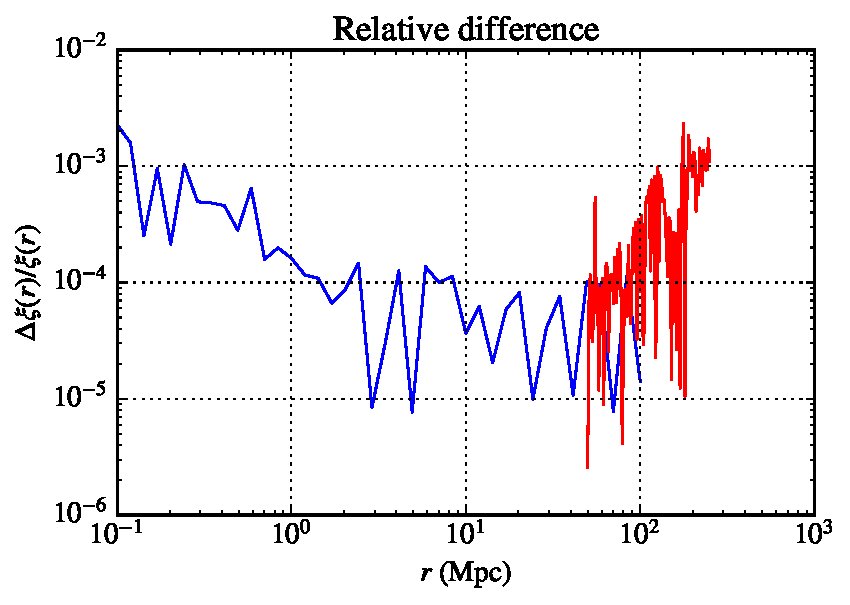
\includegraphics[width=0.47\textwidth]{benchmark_xi_rel} ~~~
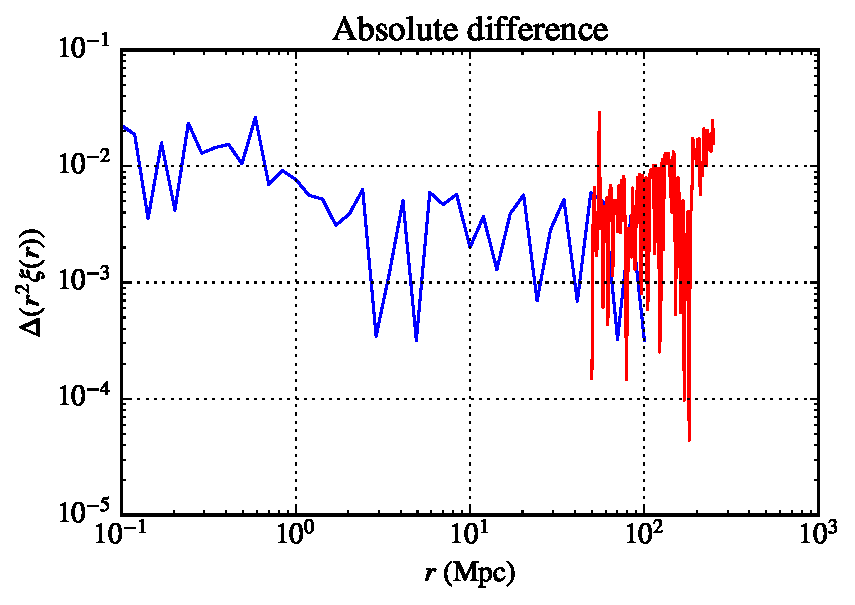
\includegraphics[width=0.47\textwidth]{benchmark_xi_abs} 
\caption{Comparison of the CCL calculation of the 3d spatial correlation function $\xi(r)$ with a precise, numerical transform of the CCL non-linear Halofit power spectrum. The left panel shows the relative error $\Delta \xi(r) / \xi(r)$. The right panel shows the absolute error in $r^2 \xi(r)$. Both panels are for the $w_a$~LCDM model of Table~\ref{table:code_comp} at redshift zero.}
\label{fig:benchmark_xi}
\end{figure*}
%
To further validate the $P(k) \to \xi(r)$ transform we performed a test using an analytical function $\xi(r) = (r / r_0)^a$, whose inverse transform $P(k)$ 
has a known analytic form. We used $r_0 = 5$~Mpc$^{-1}$ and $a = -1.67$, which gives a rough approximation to the actual 3d correlation function.   
We then compared the CCL calculation of $\xi(r)$ to the known analytic result. The relative difference $\Delta \xi(r) / \xi(r)$ was found to be   
less than 0.3\% in the range $2 < r < 250$~Mpc rising to about 5\% at $r = 1000$~Mpc (see Fig.~\ref{fig:analytic_xi}). For $r=0.1-0.8$~Mpc the relative difference is $\approx$8\%. The accuracy at low and high distances can be improved by increasing the range over which the power spectrum splines are evaluated.
%
\begin{figure*}[htbp]
\centering
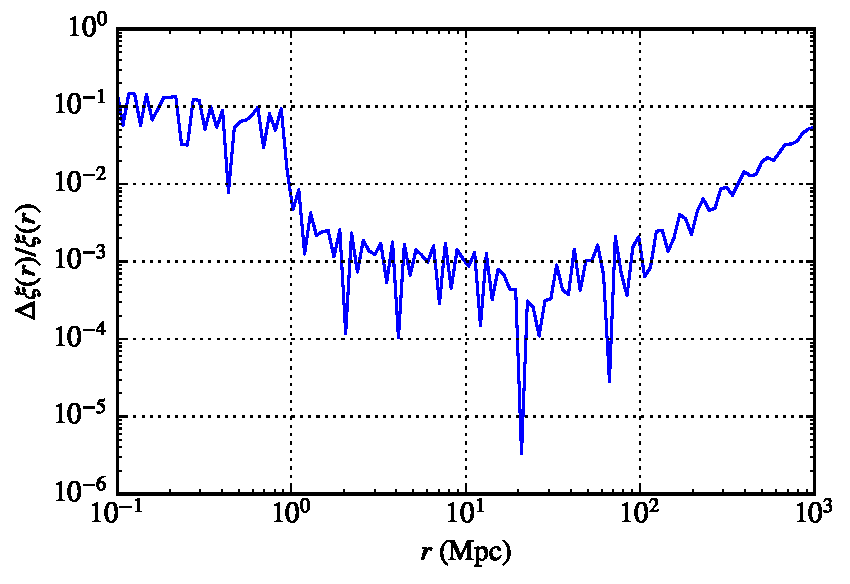
\includegraphics[width=0.47\textwidth]{analytic_xi}
\caption{The relative error in the 3d spatial correlation function computed using the CCL algorithm compared to an analytic function $\xi(r) = (r/r_0)^a$ whose inverse transform $P(k)$ is known analytically. In this validation test, the known $P(k)$ was transformed with the CCL algorithm and compared to the known analytic result for $\xi(r)$.}
\label{fig:analytic_xi}
\end{figure*}


Additionally, independent codes were utilized to test the accuracy of halo mass function predictions. For the halo mass function, we compare the value of $\sigma$, $\log(\sigma^{-1})$, and the value of the halo mass function in the form used in \cite{Tinker2008},
\begin{equation}
\log[(M^2/\bar{\rho}_m)dn/dM].
\end{equation}
We note that while we maintain the $10^{-4}$ for our evaluations of $\sigma$, the accuracy degrades to a value of $5\times10^{-3}$ for the halo mass function evaluation, primarily at the high halo mass and high redshift domains. We find that this increased error is acceptable, as the level of precision is significantly better than the accuracy of current halo mass function models.

The implementation of the matter power spectrum emulation code from \citet{Lawrence17} in \ccl has been validated at first instance by comparing the direct output of the original code to \ccl for the best fit cosmology (M000) in the range of wavenumbers spanned by the emulator predictions and confirming that the agreement is within the expectation from numerical errors (fractional difference of $<10^{-5}$). We have also compared the \ccl emulator outputs for certain cosmologies to smoothed power spectra from the simulations presented in \citet{Lawrence17}.\footnote{Courtesy of Earl Lawrence and Katrin Heitmann.} The check ensures that the \ccl outputs when calling the emulator are within $3\%$ of the simulation benchmarks at $z=0$ and for the $k$ range of validity of the emulator. This essentially corresponds to a verification of the results presented in Figure 5 and Figure 6 of \citet{Lawrence17}.

Finally, for cosmologies involving massive neutrinos, we have included tests which compare comoving distance and distance modulus predictions from {\tt CCL} from those produced by the {\tt astropy} \citep{astropy} library. In this case, we consider these comparison tests to pass if the agreement between the two predictions is 0.001 or better; this is due to the fact that {\tt astropy} uses a fitting function for the neutrino phase-space integral while we compute the integral directly. The fitting function used by astropy is expected to match the true integral at approximately this level. As a sanity check, we also include a test which verifies that the power spectrum from {\tt CLASS} as called via CCL matches that as called directly from {\tt CLASS} in three test cosmologies with massive neutrinos. 

\ccl has a suite of test routines which, upon compilation, compare its outputs to the benchmarks from code comparison. These are run with {\tt make check}.

\section{Examples for C implementation}
\label{sec:example}

Examples of how to run \ccl are provided in the {\tt tests} sub-directory of the library. The first resource for a new user should be the {\tt ccl$\_$sample$\_$run.c} file. This starts by setting up the \ccl default configuration. Then, it creates the ``cosmo'' structure, which contains distances and power spectra splines, for example. There are example calls for routines that output comoving radial distances, the scale factor, the growth factor and $\sigma_8$. Toy models are created for the redshift distributions of galaxies in the clustering and lensing samples, and for the bias of the clustering sample ($b(z)=1+z$). These are used for constructing the ``tracer'' structures via {\tt CCL$\_$Cltracer}, which can then be called to obtain the angular power spectra for clustering, cosmic shear and CMB lensing. All functions of redshift associated to each tracer can be retrieved at any arbitrary point using the same interpolation scheme used by \ccl internally.


\section{Python wrapper}
\label{sec:python}

A Python wrapper for \ccl is provided through a module called {\tt pyccl}. The whole \ccl interface can be accessed through regular Python functions and classes, with all of the computation happening in the background through the C code. The functions all support {\tt numpy} arrays as inputs and outputs, with any loops being performed in the C code for speed.

\subsection{Python installation}
\label{sec:python:install}

Before you can build the Python wrapper, you must have compiled and installed the C version of \ccl, as {\tt pyccl} will be dynamically linked to it. The Python wrapper's build tools currently assume that your C compiler is {\tt gcc}, and that you have a working Python 2.x or 3.x installation with {\tt numpy} and {\tt distutils} with {\tt swig} (the latter is not necessary for using \ccl, only for development). If you have installed \ccl in your default library path, you can build and install the {\tt pyccl} module by going to the root \ccl directory and choosing one of the following options:
\begin{itemize}
 \item To build and install the wrapper for the current user only, run \\
 {\tt \$ python setup.py install --user}
 \item To build and install the wrapper for all users, run \\
 {\tt \$ sudo python setup.py install}
 \item To build the wrapper in-place in the source directory (for testing), run \\
 {\tt \$ python setup.py build$\_$ext --inplace}
\end{itemize}
If you choose either of the first two options, the {\tt pyccl} module will be installed into a sensible location in your {\tt PYTHONPATH}, and so should be automatically picked up by your Python interpreter. You can then simply import the module using {\tt import pyccl}. If you use the last option, however, you must either start your interpreter from the root \ccl directory, or manually add the root \ccl directory to your {\tt PYTHONPATH}.

These options assume that the C library ({\tt libccl}) has been installed somewhere in the default library path. If this isn't the case, you will need to tell the Python build tools where to find the library. This can be achieved by running the following command first, before any of the commands above:

\texttt{python setup.py build$\_$ext --library-dirs=/path/to/lib/ --rpath=/path/to/lib/}

Here, {\tt /path/to/lib/} should point to the directory where you installed the C library. For example, if you ran {\tt ./configure --prefix=/my/path/} before you compiled the C library, the correct path would be {\tt /my/path/lib/}. The command above will build the Python wrapper in-place; you can then run one of the {\tt install} commands, as listed above, to actually install the wrapper. Note that the {\tt rpath} switch makes sure that the \ccl C library can be found at runtime, even if it is not in the default library path. If you use this option, there should therefore be no need to modify the library path yourself.

On some systems, building or installing the Python wrapper fails with a message similar to:

\texttt{fatal error: `gsl/gsl$\_$interp2d.h' file not found.}

This happens when the build tools fail to find the directory containing the GSL header files, e.g. when they have been installed in a non-standard directory. To work around this problem, use the {\tt --include-dirs} option when running the {\tt setup.py build$\_$ext} step above, i.e. if the GSL header files are in the directory {\tt /path/to/include/}, you would run

\texttt{python setup.py build$\_$ext --library-dirs=/path/to/install/lib/ --rpath=/path/to/install/lib/ --include-dirs=/path/to/include/}

and then run one of the {\tt setup.py install} commands listed above. (Note: As an alternative to the {\tt --include-dirs} option, you can use {\tt -I/path/to/include} instead.)

You can quickly check whether {\tt pyccl} has been installed correctly by running {\tt python -c "import pyccl"} and checking that no errors are returned. For a more in-depth test to make sure everything is working, change to the {\tt tests/} sub-directory and run {\tt python run$\_$tests.py}. These tests will take a few minutes. Notice that these are not the same tests that are run via {\tt make check}. In the case of the {\tt python} tests, the library will only check for finite outputs of the routines called from {\tt pyccl}. There is no benchmark comparison in this case.

\subsection{Python example}
\label{sec:python:example}

The Python module has essentially the same functions as the C library, just presented in a more standard Python-like way. You can inspect the available functions and their arguments by using the built-in Python {\tt help()} function, as with any Python module.

Below is a simple example Python script that creates a new {\tt Cosmology} object, and then uses it to calculate the $C_\ell$'s for a simple lensing cross-correlation. It should take a few seconds on a typical laptop.
\begin{verbatim}
import pyccl as ccl
import numpy as np

# Create new Cosmology object with a given set of parameters. This keeps track
# of previously-computed cosmological functions
cosmo = ccl.Cosmology(Omega_c=0.27, Omega_b=0.045, h=0.67, A_s=2e-9, n_s=0.96)

# Define a simple binned galaxy number density curve as a function of redshift
z_n = np.linspace(0., 1., 200)
n = np.ones(z_n.shape)

# Create objects to represent tracers of the weak lensing signal with this
# number density (with has_intrinsic_alignment=False)
lens1 = ccl.ClTracerLensing(cosmo, False, n=(z_n, n))
lens2 = ccl.ClTracerLensing(cosmo, False, n=(z_n, n))

# Calculate the angular cross-spectrum of the two tracers as a function of ell
ell = np.arange(2, 10)
cls = ccl.angular_cl(cosmo, lens1, lens2, ell)
print cls
\end{verbatim}

Further examples are collected in several Jupyter notebooks available in the {\tt examples/} directory. These are:
\begin{verbatim}
Correlation.ipynb,

Distance Calculations Example.ipynb,

HMFexample.ipynb,

Lensing angular power spectrum.ipynb,

MCMC Likelihood Analysis.ipynb,

Photo-z example.ipynb,

Correlation_3d.ipynb,

Power spectrum example.ipynb
\end{verbatim}

Note that the likelihood analysis in the last notebook is not intended to be realistic, but it gives an operational example of how {\tt CCL} can be integrated into such an analysis. In particular, the notebook only considers cosmic shear over one wide redshift bin and the covariance matrix adopted solely includes a contribution from cosmic variance. The ``data vector'' is simply a simulated using {\tt CCL} theoretical predictions. For speed, theoretical predictions use the BBKS power spectrum implementation.


\subsection{Technical notes on how the Python wrapper is implemented}
\label{sec:python:technical}

The Python wrapper is built using the {\tt swig} tool, which automatically scans the \ccl C headers and builds a matching interface in Python. The default autogenerated {\tt swig} interface can be accessed through the {\tt pyccl.lib} module if necessary. A more user-friendly wrapper has been written on top of this to provide more structure to the module, allow {\tt numpy} vectorization, and provide more natural Python objects to use (instead of opaque {\tt swig}-generated objects).

The key parts of the wrapper are as follows:
\paragraph{{\tt setup.py}} This instructs {\tt swig} and other build tools on how to find the right source files and set compile-time variables correctly. Most of this information is provided by header files and SWIG interface files that are included through the {\tt pyccl/ccl.i} interface file.

Note that certain compiler flags, like {\tt -fopenmp}, are also set in {\tt setup.py}. If you are not using {\tt gcc}, you may need to modify these flags (see the {\tt extra$\_$compile$\_$args} argument of the {\tt setup()} function).

\paragraph{Interface ({\tt .i}) files} These are kept in the {\tt pyccl/} directory, and tell {\tt swig} which functions to extract from the C headers. There are also commands in these files to generate basic function argument documentation, and remove the {\tt ccl$\_$} prefix from function names.

The interface files also contain code that tells {\tt swig} how to convert C array arguments to {\tt numpy} arrays. For certain functions, this code may also contain a simple loop to effectively vectorize the function.

The main interface file is {\tt pyccl/ccl.i}, which imports all of the other interface files. Most of the \ccl source files (e.g. {\tt core.c}) have their own interface file too. For other files, mostly containing support/utility functions, {\tt swig} only needs the C header ({\tt .h}) file to be specified in the main {\tt ccl.i} file, however. (The C source file must also be added to the list in {\tt setup.py} for it to be compiled successfully.)

\paragraph{Python module files} The structure of the Python module, as seen by the user, is organized through the {\tt pyccl/$\_$$\_$init$\_$$\_$.py} file, which imports only the parts of the {\tt swig} wrapper that are useful to the user. The complete autogenerated {\tt swig} interface can be accessed through the {\tt pyccl.lib} sub-module if necessary.

Individual sub-modules from \ccl are wrapped in their own Python scripts (e.g. {\tt power.py}), which typically provide a nicer ``Pythonic'' interface to the underlying \ccl functions and objects. This includes automatically choosing whether to use the vectorized C function or not, as well as some conversions from Python objects to the autogenerated {\tt swig} objects. Most of the core Python objects, like {\tt Parameters} and {\tt Cosmology}, are defined in {\tt core.py}. These objects also do some basic memory management, like calling the corresponding {\tt ccl$\_$free$\_$*} C function when the Python object is destroyed.

\paragraph{Auto-generated wrapper files} The {\tt swig} command is triggered when you run {\tt setup.py}, and automatically generates a number of C and Python wrapper files in the {\tt pyccl/} directory. These typically have names like {\tt ccl$\_$*.c} and {\tt ccl$\_$*.py}, and should not be edited directly, as {\tt swig} will overwrite them when it next runs.

\paragraph{{\tt pyccl/pyutils.py}} This file contains several generic helper functions for passing {\tt numpy} arrays in and out of Python functions in a convenient way, and for performing error checking and some type conversions.

The build process will also create a {\tt pyccl/ccllib.py} file, which is the raw autogenerated Python interface, and {\tt $\_$ccllib.so}, which is a C library containing all of the C functions and their Python bindings. A {\tt build/} directory and {\tt pyccl.egg-info/} directory will also be created in the same directory as {\tt setup.py} when you compile {\tt pyccl}. These (plus the {\tt pyccl/$\_$ccllib.so} file) should be removed if you want to do a clean recompilation. Running {\tt python setup.py clean --all} will remove some, but not all, of the generated files.


\section{Future functionality to be included}
\label{sec:future}

In the future, we hope that \ccl will include other functionalities. Functionalities which are currently under development:
\begin{itemize}
        \item a link to {\tt angpow} \citep{2017arXiv170103592C} for going beyond the Limber approximation,
	\item a link to {\tt FAST-PT} \citep{FASTPT} for efficient implementation of nonlinear perturbation theory,
	\item and more power spectrum methods (see \ref{Pk_wishlist}).
\end{itemize}

\section{Feedback}
\label{sec:feedback}

If you would like to contribute to \ccl or contact the developers, please do so through the \ccl github repository located at \url{https://github.com/LSSTDESC/CCL}.

\section{Citing \ccl}
\label{sec:cite}

If you use \ccl in your work, please provide a link to the repository and cite it as LSST DESC (in preparation). For free use of the {\tt CLASS} library, the {\tt CLASS} developers require that the {\tt CLASS} paper be cited: {\it  CLASS II: Approximation schemes}, D. Blas, J. Lesgourgues, T. Tram, arXiv:1104.2933, JCAP 1107 (2011) 034. The {\tt CLASS} repository can be found in \url{http://class-code.net}.

\section{License}
\label{sec:license}

Copyright \textcopyright 2017, the LSSTDESC \ccl contributors are listed in the
documentation (``research note'') provided with this software. The repository can be found at \url{https://github.com/LSSTDESC/CCL}. All rights reserved.

Redistribution and use in source and binary forms, with or without
modification, are permitted provided that the following conditions are met:

\begin{itemize}
\item Redistributions of source code must retain the above copyright notice, this
  list of conditions and the following disclaimer.
\item Redistributions in binary form must reproduce the above copyright notice,
  this list of conditions and the following disclaimer in the documentation
  and/or other materials provided with the distribution.
\item Neither the name of \ccl (\url{https://github.com/LSSTDESC/CCL}) nor the names of its
  contributors may be used to endorse or promote products derived from
  this software without specific prior written permission.
\end{itemize}

THIS SOFTWARE IS PROVIDED BY THE COPYRIGHT HOLDERS AND CONTRIBUTORS ``AS IS''
AND ANY EXPRESS OR IMPLIED WARRANTIES, INCLUDING, BUT NOT LIMITED TO, THE
IMPLIED WARRANTIES OF MERCHANTABILITY AND FITNESS FOR A PARTICULAR PURPOSE ARE
DISCLAIMED. IN NO EVENT SHALL THE COPYRIGHT HOLDER OR CONTRIBUTORS BE LIABLE
FOR ANY DIRECT, INDIRECT, INCIDENTAL, SPECIAL, EXEMPLARY, OR CONSEQUENTIAL
DAMAGES (INCLUDING, BUT NOT LIMITED TO, PROCUREMENT OF SUBSTITUTE GOODS OR
SERVICES; LOSS OF USE, DATA, OR PROFITS; OR BUSINESS INTERRUPTION) HOWEVER
CAUSED AND ON ANY THEORY OF LIABILITY, WHETHER IN CONTRACT, STRICT LIABILITY,
OR TORT (INCLUDING NEGLIGENCE OR OTHERWISE) ARISING IN ANY WAY OUT OF THE USE
OF THIS SOFTWARE, EVEN IF ADVISED OF THE POSSIBILITY OF SUCH DAMAGE.

%
This paper has undergone internal review in the LSST Dark Energy Science Collaboration. We thank the reviewers: Yao-Yuan Mao, Mariana Penna-Lima and Mike Jarvis for comments that halped improved this manuscript and the \ccl library overall. 

%DESC standard paper acknowledgements
%From https://github.com/LSSTDESC/desc-tex/blob/master/ack/standard.tex
The DESC acknowledges ongoing support from the Institut National de Physique Nucl\'eaire et de Physique des Particules in France; the Science \& Technology Facilities Council in the United Kingdom; and the Department of Energy, the National Science Foundation, and the LSST Corporation in the United States.  DESC uses resources of the IN2P3 Computing Center (CC-IN2P3--Lyon/Villeurbanne - France) funded by the Centre National de la Recherche Scientifique; the National Energy Research Scientific Computing Center, a DOE Office of Science User Facility supported by the Office of Science of the U.S.\ Department of Energy under Contract No.\ DE-AC02-05CH11231; STFC DiRAC HPC Facilities, funded by UK BIS National E-infrastructure capital grants; and the UK particle physics grid, supported by the GridPP Collaboration.  This work was performed in part under DOE Contract DE-AC02-76SF00515. 

%In addition
We would like to thank the organisers of the the DESC meetings at: CMU (July 2018), Oxford (July 2016), SLAC (Ferurary 2018, March 2016), and ANL (2015), and the LSST-DESC Hack Week organisers (CMU, November 2016), where this work was partly developed. We would also like to acknowledge the contribution of the participants of the Theory and Joint Probes Code Comparison Project, some of whom are among the \ccl contributors, for providing the benchmarks for testing CCL. We also acknowledge Louis Penafiel and Elizabeth Kimura, who developed the {\tt VARRIC} code to compare and visualize power spectra calculated by {\tt CCL} and {\tt CLASS}. Finally, we are grateful for the feedback received from other working groups of DESC, including Strong Lensing, Supernovae, Clusters and Photometric Redshifts.
We thank Peter Williams for making his ApJ bibstyle file available at \url{https://github.com/pkgw/tex-stuff/blob/master/yahapj.bst}. We are grateful to Katrin Heitmann and Earl Lawerence for discussions concerning the Cosmic Emulator. We are also thankful to the {\tt CLASS} authors and to Andrew Hamilton for making their codes available and allowing us to use them in this work. 
%

DA is supported by the Science and Technology Facilities Council (STFC) through an Ernest Rutherford Fellowship, grant reference ST/P004474/1. NEC acknowledges support from a Beecroft fellowship and a Royal Astronomical Society Research Fellowship. TT acknowledges funding from the European Union's Horizon 2020 research and innovation programme under the Marie Sk{l}odowska-Curie grant agreement No.\ 797794.MI acknowledges support by NSF under grant AST-1517768.


Author contributions are listed below. \\
Husni Almoubayyed: wrote an mcmc jupyter notebook example, reviewed code/contributed to issues. \\
David Alonso: Co-led project; developed structure for angular power spectra; implemented autotools; integrated into LSS pipeline; contributed to: background, power spectrum, mass function, documentation and benchmarks; reviewed code \\
Jonathan Blazek: Planning capabilities and structure; documentation and testing. \\
Philip Bull: Implemented the Python wrapper and wrote documentation for it; general bug fixes, maintenance, and code review; enhanced the installer and error handling system. \\
Jean-\'Eric Campagne: Angpow builder and contributed to the interface with CCL. \\
N. Elisa Chisari: Co-led project, coordinated hack projects \& communication, contributed to: correlation function \& power spectrum implementation, documentation, and comparisons with benchmarks. \\
Alex Drlica-Wagner: Helped with document preparation. \\
Zilong Du: Implemented the 3d correlation function, redshift-space correlation functions, and corresponding benchmarks. \\
Tim Eifler: Reviewed/tested code. \\
John Ellison: Implemented the 3d correlation function, redshift-space correlation functions, and corresponding benchmarks; wrote text describing 3d and redshift-space correlation functions for this note. \\
Ren\'ee Hlozek: Contributed initial code for error handling structures, reviewed other code edits. \\
Mustapha Ishak: Contributed to planning of code capabilities and structure; reviewed code; identified and fixed bugs. \\
Shahab Joudaki: Created physical density function and documentation. \\
Matthew Kirby: Performed comparison of physical constants. \\
David Kirkby: Writing, testing and reviewing code. Asking questions. \\
Elisabeth Krause: Initiated and co-led project; developed CLASS interface and error handling; contributed to other code; reviewed pull requests. \\
Francois Lanusse: Worked on install procedure \\
C. Danielle Leonard: Wrote and tested code for LSST specifications, user-defined photo-z interface, and support of massive neutrinos; reviewed other code; wrote text for this note. \\
Christiane S. Lorenz: Contributed to accurate high-redshift cosmological background quantities and benchmarked background splines. \\
Phil Marshall: Helped with document preparation. \\
Thomas McClintock: Wrote Python documentation. \\
Sean McLaughlin: Wrote doxygen documentation and fixed bugs/added functionality to distances. \\
Alexander Mead: Wrote halo model code \\
J\'er\'emy Neveu: Contributed to Angpow and built the interface with CCL. \\
St\'ephane Plaszczynski: Contributed to Angpow and contributed to the interface with CCL. \\
Javier Sanchez: Modified setup.py to allow pip installation and uninstall. \\
Sukhdeep Singh: Contributed to the correlation functions code. \\
An\v{z}e Slosar: Wrote and reviewed code. \\
Tilman Tr\"oster: Wrote code for user-changable precision parameters, added distance and growth factor tests, found and fixed bugs. \\
Antonio Villarreal: Contributed to initial benchmarking, halo mass function code, and general code and issues review. \\
Michal Vrastil: Wrote documentation and example code, reviewed code. \\
Joe Zuntz: Wrote initial infrastructure, C testing setup, and reviewed code. \\


%{\it Facilities:} \facility{LSST}

\bibliography{main}

\end{document}
%
